%==================================================================================================
%   LUKES THESIS TEMPLATE 1.2
%   -------------------------
%   This template is based upon the offcial IMM PhD Thesis template, it is enhanced with a number
%   of new features and a number of errors have fixed. This template is intended to be complied to
%   PDF using PDFLATEX and is tested using the MiKTeX 2.9 LaTeX distribution.
%   It is based on the official DTU-IMM Thesis template by Finn Kuno Christensen in 2009.
%   Small bugfixes by Kasper Laursen in 2012.
%   -------------------------
%   Last Updated: 2012-09-19
%   Contact: lthhe@imm.dtu.dk
%==================================================================================================
%
%==================================================================================================
% DOCUMENT SETUP
%==================================================================================================
\documentclass[10pt,twoside]{book}                  %Official DTU-IMM Thesis document setup
%
%Set to 'print' for printed version, use 'net' for online version
\def\thesisversion{print}
%
%==================================================================================================
% PACKAGES
%==================================================================================================
\usepackage{LukeThesis}                             %Import Thesis base style
%input{PhDMacros}                                   %Thesis specific macros
%
%==================================================================================================
% THESIS PROPERTIES (Modifiy these fields with your details)
%==================================================================================================
\def\thesisauthor{Luke Herbert}                     %Author
\def\thesistitle{Something something}               %Title
\def\thesishandin{01-January}                       %Submission date (Day-Month}
\def\thesisdegree{PhD}                              %Degree ('B.Eng', 'B.Sc.', 'M.Sc.' or 'PhD')
\def\thesisyear{2012}                               %Submission year
\def\thesisnumber{????}                             %DTU-IMM Serial number (do not include year)
\def\thesisISSN{0000-0000}                          %ISSN number
\def\thesiskeywords{Keywords are, comma separated}  %PDF keywords
\derivethesisprops                                  %Derive dependent properties
%
%==================================================================================================
% SECTION NUMBERING SETUP
%==================================================================================================
\setcounter{tocdepth}{2}                            %2 adds sections up to subsections
\setcounter{secnumdepth}{3}                         %Subsubsections get a number when this is 3
%
%==================================================================================================
% THESIS STRUCTURE  (Modifiy to include more chapters etc)
%==================================================================================================
\begin{document}
%------------------------
%Pre-frontmatter material
%------------------------
\prefrontmatter
%--------------------
%Frontmatter material
%--------------------
\frontmatter
\pagenumbering{roman}                               %Set frontmatter numbering style
\chapter{Summary (English)}

In this report we will document our efforts to develop the Xmas (cross platform Multi-Agent System) engine for designing MAS (Multi Agent System) environments and managing intelligent agents acting in them. As the engine is for designing environments, the agents are supposed to receive commands from and send percepts to a seperate agent programming language, which implements the artificial intelligence of the agents. 

The primary goal of the project is to make the engine as general as possible so as to allow any desirable environment to be designed with it, while making it easy to extend individual components to suit the needs of specific types of MASs. The engine comes packaged with support for interfacing with EIS (Environment Interface Standard), and, by extension, the agent programming languages supported by it. A simple tile-based environment is also provided. The engine is designed with the model-view-controller (MVC) pattern, to allow clear seperation of components. To showcase and test our engine, we have created a reference implementation which uses the GOAL agent programming language to control agents.

We believe that the Xmas engine have achieved a high degree of generality, although this comes at the expense of features and functionality useful to many MASs, which have instead been delegated to extensions. The engine is best suited for designing, setting up and executing larger systems, as there is a lot of overhead involved. The engine as well as the example extensions runs on the major operating systems, including Linux, Windows and Mac OS.                                   %English summary of Thesis
\markboth{}{}                                       %Set headings (left)(right)
\chapter{Summary (Danish)}
\begin{otherlanguage}{danish}

Målet for denne afhandling er at ...

\end{otherlanguage}                                   %Danish summary of Thesis
\markboth{}{}                                       %Set headings (left)(right)
\chapter{Preface}

This thesis was prepared at the department of Informatics and Mathematical Modelling at the Technical University of Denmark in fulfilment of the
requirements for acquiring an M.Sc. in Informatics.

The thesis deals with ...

The thesis consists of ...
%==================================================================================================
% SIGNATURE AREA
%==================================================================================================
\vspace{20mm}
\begin{center}
    \hspace{20mm} Lyngby, \thesishandin-\thesisyear
    \vspace{5mm}
    \newline
  %Update signature image file in line below
    
\includegraphics[scale=0.5]{figures/SignatureDummy}
\end{center}
\begin{flushright}
    \thesisauthor
\end{flushright}
% % % EOF % % %                                     %Preface
\markboth{}{}                                       %Set headings (left)(right)
\chapter{Acknowledgements}

I would like to thank my....

                            %Acknowledgements
\markboth{}{}                                       %Set headings (left)(right)
%------------------
% Table of contents
%------------------
\newpage\mbox{}\newpage
\chaptermark{Contents}
\pdfbookmark{\contentsname}{toc}
\renewcommand{\sectionmark}[1]{\markright{#1}}
\sectionmark{Contents}
\addtolength{\parskip}{-\baselineskip}
\tableofcontents
\addtolength{\parskip}{\baselineskip}
\renewcommand{\sectionmark}[1]{\markright{\thesection\ #1}}
%-------------
% Main content
%-------------
\mainmatter
\pagebreak{}



\chapter{Introduction}


\subsection{Motivation}

There are many complications when developing multi agent systems,
our goal with this project was to lessen one of these by designing
an engine with the specific purpose to develop multi agent environments.
What these environments can be is left to the developer, however almost
everything in the engine is modular and interchangeable, ensuring
that all types of multi agent environments are possible. 

What the types of projects can be is manyfold but here are some possible
examples:


\paragraph*{Agent comparison software }

There are many different languages in which it is possible to write
agent programs, some are specifically designed for it others are powerful
enough to accommodate the possibility of agent programming. Our engine
is designed with support for multiple languages at once which makes
this engine a perfect candidate for designing a comparator program. 

For instance, if two groups wanted to test their agent programs against
each other, this engine would make it possible for them to easily
design a world in which this test could occur.


\paragraph*{Agent testing/Simulation software}

Testing agent software can be complicated. Being able to rapidly create
an environment and visualize it can be important to the project, as
it ensure basic mistakes are ironed out before larger scale implementation. 


\paragraph*{Agent teaching tools}

Teaching agent languages can be tough without proper exercises; however,
the time spent on designing these exercises can prove too exhausting
for the teacher to develop. In this case the teacher can rapidly design
the world he had in mind for his exercise instead of designing every
integral part of the multi agent system himself. This is because our
engine provides all the basic features of a multi agent system, so
that the time can be spent more productively on designing how a given
exercise should play out, showcasing the problem the students are
supposed to deal with.


\paragraph*{Computer games}

In theory most computer games are just multi agent programs where
one of the agents is controlled by the player. Our engine should make
it fairly easy for setting up a framework for creating rules inside
a given world and ensure that the agents of the world follow said
rules. \texttt{\emph{{[}Expand{]}}}



\chapter{Theory}


\section{Multi-Agent Systems}


\subsection{Agents and Environments in Artificial Intelligence}

In artificial intelligence, an agent is something that can perform
actions in and (partially or fully) perceive the state of the environment
it is situated in. As an example, consider an agent tasked with finding
the shortest route between two nodes in a weighted, undirected graph,
with the limitation that it can only see the nodes that have an edge
to the one it is standing in. We will now use this example to describe
what (Russel, Norvig, 2010) calls a \emph{task environment}, consisting
of definitions for the performance measure for the agent, the environment
it acts in, the actions it can take, and its facilities for perception:
\begin{description}
\item [{Environment}] The environment is a model of the world the agent
acts in. In our example, it is described as a graph. The environment
may also contain artifacts for agents to interact with, such as a
packages to pick up or obstacles to navigate around.
\item [{Actions}] This denotes what actions the agent can take to change
the state of the environment or itself. In the example, the agent
would have a \emph{move} action, allowing it to move to an adjacent,
connected node.
\item [{Percepts}] If the agent is to make intelligent decisions, it must
be able to perceive the current state of the world -- that is, itself
and the environment. Such a fragment of information that the agent
have sensed is called a percept. In the running example, the agent
can perceive the nodes immediately connected to the one it is standing
on, as well as the edges to those nodes.
\item [{Performance}] For an agent to be as efficient as possible, it is
useful to have a performance measure describing how well the agent
is executing the task at hand. In the provided example, the performance
measure could be defined in terms of the number of actions taken per
unique node visited, giving the agent an idea of the amount of redundancy
in its pathfinding.
\end{description}
While the task environment can be used to succinctly describe the
properties of the world, it says nothing of the logic that the agent
applies to perform tasks in the world. This is left in the hands of
an \emph{agent program}, which is responsible for processing the percepts
and choosing actions for an agent. In general, an agent program receives
percepts and chooses an appropriate action based on the knowledge
available to it in an aptly named \emph{percept-action} \emph{cycle}.
This knowledge may just be the current percepts, or it may be all
the percepts retreived so far. When choosing an action, it may take
into consideration how different actions would affect the world, and
how much closer performing the action would bring the agent to its
goal. Agents with such capable agent programs are called \emph{utility-based
agents} in (Russel, Norvig, 2010).


\subsection{Multi-Agent Systems}

While there is no strict, universal definition of what constitutes
a multi-agent system, the following seems to represents the simplest
consensus: \emph{In a multi-agent system, several intelligent agents
act and interact more or less autonomously in an environment}. The
interacting of agents may be of any character, the important part
is that each agent can be aware of the others and affect their execution
directly or indirectly. Here, a direct effect means changing another
agents state, eg.\ by moving it into another postition or decreasing
its health. An indirect effect could be communicating with the agent,
suggesting another execution path. As such \texttt{\emph{{[}unclear?{]}}},
a system in which agents compete for ressources and hinder other agents'
progress is a multi-agent system, as is a system in which the agents
work together towards a common goal. 

While the former may be useful in simulating certain systems, the
latter is more interesting in software design, as such an approach
could conceivably lead to more decentralized problem solving. A mixture
of the two approaches can also be used, as in the Multi-Agent Programming
Contest \texttt{\emph{{[}Link{]}}}, where teams of cooperating agents
compete for points. In this case, the goal for each team is to develop
the best strategy, where performance is measured by competitiveness.

In addition to the above, limiting the agents' knowledge of the state
of the world is a desirable characteristic of a MAS; otherwise, there
would be no need for the agents to communicate, and they could just
as well be subroutines of a single agent (Panait and Luke, 2005).
It could still be modelled as a MAS, of course, but not a very interisting
one \texttt{\emph{{[}rewrite sentence{]}}}. Additionally, the case
could be made that the less agents know of the world, the less information
they have to process when searching for an action to execute, thus
reducing their computational load. On the other hand, less information
can cause the agent to follow a suboptimal execution path, causing
a trade-off between computation time and optimality. 

One of the strong points of multi-agent systems is that it consists
of several pieces of software running more or less autonomously. As
mentioned above, this allows for developing decentralized systems,
where agent programs runs on different threads or servers. In the
context of distributed systems, less dependency on a central intelligence
is of course preferred. Furthermore, MASs are useful when simulating
naturally occuring systems wherein several ``agents'' interact with
each other, such as a group of different animals around a watering
hole or costumers in a store. \texttt{\emph{{[}sentence out of context{]}}}


\subsection{The GOAL Agent Programming Language}

\texttt{\emph{{[}Reference to the GOAL manual{]}}}

Several APLs (Agent Programming Languages) have been developed to
suit the defining characters of agents and their interaction with
environments as we have described them above. In this section, we
will focus on the relatively new GOAL APL, which can be written using
the prolog logic programming language.

In GOAL, code is segmented into sections describing:
\begin{itemize}
\item What it knows
\item What it wants to achieve
\item What it can do
\item How it handles new information (percepts) from the environment
\item The actual logic for choosing an appropriate action to execute
\end{itemize}
The first two points in the list will be explained below. 


\subsubsection*{Mental State}

GOAL provides the notion of \emph{mental state} of an agent, which
describes what the agent knows and what it aims to achieve. Specifically,
it consists of the following three components:
\begin{description}
\item [{Knowledge}] describes what the engine knows to be universally true.
This information is completely static; it is something the agent is
``born'' with, and can not be changed. In other words, this describes
the rules and constants of the system.
\item [{Beliefs}] are facts the agent deduces during its execution, using
its knowledge. Beliefs can be updated at runtime by using the \texttt{insert($\varphi$)}
and \texttt{delete($\varphi$)} commands, where\texttt{ $\varphi$}
is a belief. The \texttt{bel($\varphi$)} operation can be used to
ascertain whether the agent believes that $\varphi$.
\item [{Goals}] are what the agent strives to accomplish. These can be
dynamically updated along the way to acommodate a changing world.
This is done with the \texttt{adopt($\varphi$)} and \texttt{drop($\varphi$)}
commands, where $\varphi$ is a goal. \texttt{goal($\varphi$)} checks
whether $\varphi$ is currently a goal of the agent. If a goal have
been achieved -- that is, if the agent's current beliefs and knowledge
satifies a goal -- it is automatically removed from the \texttt{goals}
collection, as the agent would otherwise keep trying to accomplish
it. 
\end{description}
The information in the mental state is stored as logical statements
in prolog. The operations mentioned above for querying and modifying
the mental state thus takes a prolog statement as input.


\subsubsection*{Acting and Perceiving}

When a GOAL program is run, it executes the following steps, in order:
\begin{enumerate}
\item Receive percepts
\item Update the goals and beliefs of the agent if needed
\item Choose an appropriate action to execute
\end{enumerate}
This is repeated in a cycle. 

The processing of new percepts mentioned in point \#2 is handled in
the \texttt{event module} of the agent program. Here, all new percepts
in the current cycle can be inspected, and the mental state of the
agent can be updated. If, for example, the agent perceives that it
is in a different location than in the previous cycle, this module
can be used to change its beliefs accordingly. If the world have changed
drastically, the agent may also choose to drop goals that can no longer
be achieved, and/or adopt goals that seems more fruitful to pursue.
As such, the processing of percepts is the primary place to change
the mental state of the agent.

The choosing of an action is where the agent decides -- based on its
mental state -- which execution path it should take. The actions themselves
are provided in an \texttt{action specification} section of the program,
where each action denotes pre- and postconditions of the action. That
is, what must hold for the action to be executed and what effect it
will have on the environment. An action is not considered for execution
if its precondition does not hold. If it does hold and the action
is taken, the logical statements in the postcondition is inserted
into the belief base. 

When an action have been chosen in GOAL, it is only \emph{set} to
be executed, that is, GOAL requests that it be executed. It might
be that the program managing the agent in the environment sees fit
to not execute it, or that the action fails (if the agent tries to
move into a wall, for example). In that case, GOAL only knows about
the failure of the action if it is somehow obvious from the next set
of percepts it receives. In light of this, postconditions on actions
should only be used when it absolutely certain that what the postcondition
specifies is true, as it may otherwise insert flawed information into
the agents beliefs.


\subsection{The Environment Interface Standard}

Several agent programming languages -- including GOAL -- is only concerned
with the agent logic of a MAS. To provide a world in which these agents
can function, they need to be connected to a program providing an
environment. \texttt{\emph{{[}Reference EIS technical report{]}}}

EIS (Environment Interface Standard) is a tool which can be used to
design environments and connect them to agent programming languages.
As such, it does not assume much about the implementation of the environments
or the agents inhabiting it. It provides \texttt{entities} which can
function as the bodies of agent programs, and means for receiveing
commands and returning percepts to the connected agents.

When using EIS, the environment designer can handle actions sent by
the agent programs with the \texttt{performAction} method to define
exactly how they affect the world the designer have constructed. Percepts
can be requested explicitly through the \texttt{getAllPercepts} method
(this is how GOAL gets its percepts from EIS) or as notifications,
for APLs that support it. 

The main point of EIS is to provide a standard (hence the name) for
developing MASs, such that environments designed with this standard
can easily be interfaced with different APLs. As such, EIS comes pre-loaded
with bindings for several common APLs such as GOAL and Jason. As part
of this standard, the IILang (Interface Immediate Language) abstract
syntax tree have been developed. It can be used to easily and unambiguously
define actions and percepts consisting of identifiers, numerals, representations
of functions over identifiers and numerals, and lists of identifiers,
numerals and functions. These IILang objects can be created as native
Java objects and easily parsed to -- in the case of GOAL -- prolog
statements, and vice versa.

In conclusion, it is important to note that GOAL and EIS are supposed
to be two components of a multi-agent system. GOAL is not supposed
to maintain an environment, and EIS is not very well suited for implementing
agent logic.


\subsubsection*{References}

Stuart J. Russel, Peter Norvig, ``Artificial Intelligence: A Modern
Approach'', Prentice Hall, Upper Saddle River, New Jersey 07458,
3rd ed., 2010\\


Panait, Luke, ``Cooperative Multi-Agent Learning: The State of the
Art'', Autonomous Agents and Multi-Agent Systems, Volume 11, Issue
3, pp.\ 387-434, 2005.



\subsection{Model View Controller}

To ensure that code is correctly decoupled from one another, strict
design patterns are necessary, as these allow developing complex projects
without losing the sight of the entire project. If no pattern is followed,
code can easily become so entangled that later development might prove
impossible. This section will cover all the rules and ideas behind
the MVC (Model-View-Controller) design pattern.

The MVC pattern principle is that programs that can be interacted
with by a user can be split into three different components. These
components are as follows:
\begin{itemize}
\item Model -- Core of the program
\item View -- Visualization of the program
\item Controller -- Manager of state changes to the core of the program
\end{itemize}
\begin{figure}
\centering{}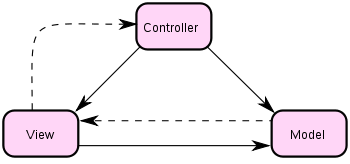
\includegraphics{MVC}\caption{\label{fig:MVCBasic}This image shows how the three components are
connected to each other; the full arrows indicate that a component
has complete knowledge of the component it is pointing to. A dashed
arrow indicates that the component the dashed arrow is pointing to
is listening to the component the arrow is originating from. }
\end{figure}



\subsubsection{Model}

The model is the core of the program. It is why the program functions
as it does, it contains all information of the data, and it is here
all business logic is located. The model should have no knowledge
of either the view or the controller; by not knowing either the program
is ensured to not be tainted by their influence.

While it may not know of the view or the controller, it is paramount
that the model is built to optimally transfer information concerning
its current state. That means that providing a way for other components
to listen on the model is very welcome\emph{. }This gives the model
a way to publish its state when it has been altered\emph{.} What this
does for the model is that in the case that model state has been altered,
it will have a way to provide the information of the state. 

If such features are not built into the model then it would require
the component changing the state to inform of the state changes, in
case of a MVC design. The component changing state is the controller
and such the controller would both have the duty of changing the state
and maintaining the view. This is generally the case of a badly designed
model and can be completely avoided if the model simply has the ability
to inform its listeners of any changes.


\subsubsection{View}

The view is a way to visualize what is currently occurring inside
model by visualizing it to the user. A view may take many shapes depending
on the model. If, for instance, the model is a program crunching data
on a server, then the view could take the form of a logging console.
Or if the model was a computer game then the view would be the graphic
representation of the game. Additionally, a model can have severl
views, each displaying information in a different manner. For example,
the computer game mentioned above could also feature a view printing
debugging information to a console while the game was running. Generally,
a view should only have knowledge of the model and not the controller.
The idea is that if the model data is complete then interaction with
the controller should not be necessary.

When designing a view there are some common pitfalls that happen easily
if one is not careful of the design. First off, the view is what it
is named; a view. This means that it should never do any state changes
to the model. If getting hold of data means that the model must change
its state to accommodate this, then the model is poorly made and should
be changed. However, a view is allowed to change its own state without
involving either the controller or model. To fully understand what
is meant by this, consider the following example:

Assume you have a menu bar as depicted in fig. \ref{fig:menubar}.

\begin{figure}[H]
\begin{centering}
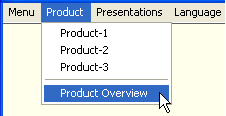
\includegraphics{MenuBar}
\par\end{centering}

\caption{\label{fig:menubar}A standard menu bar.}
\end{figure}


To open a menu, the user need to drag the mouse and click on one menu
he or she wishes to open. Many would see this as a task of the controller.
This is not the case, however, since the changes done are only performed
on the view's own state and not the model of the program.


\subsubsection{Controller}

The controller is the link between the model and the user. By convention,
all changes the user wishes to perform on the model should be done
through the controller. Like the view, it can take many shapes, like
an object that transforms input from the mouse into changes to the
model, or an object controlling how a network data stream effects
on the model. 

In a well-designed program the controller should never have to interact
with the view. However, this can be practically impossible on larger
projects unless they are carefully planned, and as such the controller
by convention is allowed to know of both the view and the model.

A common mistake when designing the controller is to mistake the unit
which the controller gets input from as the actual controller. In
many cases, the keyboard is the device from which input is transformed
into state changes to the model. However, that does not mean that
the controller should be the only unit interacting with the keyboard.
Going back to the example used to understand the view, the reason
why the controller should not deal with opening a menu bar on the
view is because the controller is not responsible of the state of
the view. The controller is only responsible for the state of the
model; the only case in which it is allowed for the controller to
interfere with the view is in the case that the model was unsuccessful
in properly informing about its state change caused by the controller.
In this case it is okay for the controller to call the view and ask
it to adjust itself. 

The reasoning for why the controller is normally mistaken to be responsible
for handling changes to the state of the view is because it is mistakenly
thought of as a controller for the entire program and not the model,
a view may contain its own controller which should not be mistaken
from the other controller. To fully understand this, imagine that
the view in itself also contains a MVC inside itself (see fig. \ref{fig:MVCeption}).

\begin{figure}[h]
\begin{centering}
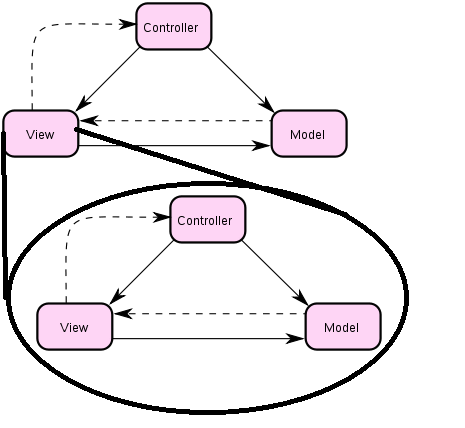
\includegraphics[width=0.6\textwidth]{MVCeption}
\par\end{centering}

\caption{\label{fig:MVCeption}A view with a MVC inside of it.}
\end{figure}


The model of a view (such as a menu bar) would contain data about
the names of the menus and it would be responsible for ordering and
accessing information as to what each menu contains. Its view would
be that of a drawing board responsible for properly drawing the menu
bars. Luckily, most views are simple, so one does not need to make
an entire MVC design, but for graphical user interface used in most
operating system it is very important to understand that a view can
be an entire MVC setup in itself. This is why most operating system
comes with libraries to easily design GUI.









\chapter{Reference Implementation}

In this section we will introduce our reference implementation (henceforth
sometimes called the \emph{package grabber scenario}), which we have
developed to showcase and test our engine. It will also serve as an
example of using the engine as well as the extensions we have provided.
In section \ref{sec:ImplementationReferenceImplementation}, we will
detail the actual implementation of the scenario in the engine, the
agent programs, as well as the integration of the two. A less complex
example, which describes the simple vacuum world (~\cite{Norvig96},
p.\ 35), can be found in appendix\texttt{\emph{ \ref{chap:VacuumWorldAppendix}}}.

The reference implementation is intended to cover as many of the engine
features and extensions as possible, while not focusing on creating
any particularly revolutionary artificial intelligence. As such, we
have set up a world that is relativively simple with respect to the
action and perception repetoire of the agents, and with an environment
representation limited in complexity. Thus, the interesting part of
the reference implementation is not the scenario itself, but rather
the actual implementation. That being said, the scenario is as follows:

\begin{figure}
\begin{centering}
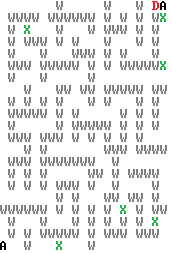
\includegraphics[width=0.4\textwidth]{TileWorldColoredScrot}
\par\end{centering}

\caption{An initial configuration of the package grabber scenario. \texttt{D}
(red) marks the dropzone, \texttt{X}s (green) are packages, \texttt{A}s
(black) are agents and \texttt{W}s (grey) are walls\label{fig:maze-scrot}}
\end{figure}


The agents in the scenario are tasked with exploring a maze in a discrete
two dimensional grid of tiles in order to locate \texttt{package}s
and bring them to a special tile called the \texttt{dropzone} (see
figure \ref{fig:maze-scrot}). A tile in this scenario can contain
several objects, unless they are explicitly forbidden to occupy the
same square. An agent, for example, can not move into a tile that
already contains another agent, but it can move into a square containing
a package or a dropzone. Importantly, a tile containing a \texttt{wall}
cannot contain anything else, thus the tiles between walls constitutes
the navigable pathway of the maze. 


\subsection*{Actions}

The three actions \emph{moving}, \emph{grabbing} and \emph{dropping}
are enough for the agents to fulfill their task, and as such they
describe the complete action specification:
\begin{description}
\item [{\texttt{move(}\texttt{\emph{Direction}}\texttt{)}}] moves the agent
one tile in the specified \texttt{\emph{Direction}}. \texttt{\emph{Direction}}\emph{
}is limited to the four cardinal directions, so an agent can only
move to an immediately adjacent square. Note that every tile not containing
a wall is reachable from every other such tile in the maze when following
this movement rule.
\item [{\texttt{grab}}] removes the package in the same tile as the agent
(if any) from the world, and marks the agent as carrying a package.
\item [{\texttt{drop}}] adds a package to the world in the same tile as
the agent (if it is carrying a package) and marks the agent as not
carrying a package. If a package is dropped at a dropzone, it is removed
from the world.
\end{description}
Note that this action specification does not mention any means of
communicating or otherwise cooperating, which is an otherwise important
feature of any multi-agent system. We have not implemented such functionality
in the XMAS engine, although it would be a high priority task if we
were to develop it further. Normally, GOAL provides built-in communication
devices, which we cannot use in the reference implementation, for
reasons explained in the implementation section{[}NOT THAT SURE{]}.
In general, although several grabber agents can inhabit the scenario,
they will not actively work together or compete, although they will
try to accomplish the same goals.


\subsection*{Percepts}

\begin{figure}
\begin{centering}
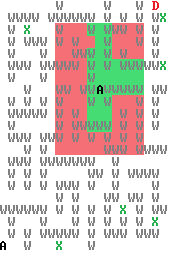
\includegraphics[width=0.4\textwidth]{TileWorldColoredScrotVision}
\par\end{centering}

\caption{Here we see the visible tiles for the agent in the middle of the colored
section. Tiles colored in green are visible to the agent while tiles
in red are are blocked by walls. All other tiles are outside the agents
visibility range, and thus invisible. As can be seen, agents are good
at peeking around corners.\label{fig:maze-scrot-vision}}


\end{figure}


Now that agents can act in the environment, they must also be able
to sense their surroundings in order to make informed choices about
their course of action. For this purpose, the following three percepts
can be obtained from the world:
\begin{description}
\item [{Vision:}] A rather obvious perception device in this scenario is
\emph{vision}, allowing an agent to learn the contents of tiles around
it. Each agent can can see a distance of five tiles in any direction,
assuming there is no walls or other agents blocking its vision. See
fig. \ref{fig:maze-scrot-vision} for an illustration.
\item [{Package~Possession:}] Specifies whether the agent is currently
holding a package. An agent can only hold one package at a time. This
truth value could be mangaged by the agent program, but having it
as a percept is easier on the AP. Additionally, an effect could forcibly
remove a package from an agent, and we would thus need a percept for
that (note that such an effect does not currently exist in the scenario).
With our current approach, we provide a snapshot of the state of the
perceivable world through percepts and let the AP make of it what
it can.
\item [{Position:}] The absolute position of the agent in the grid. In
the agent program, we initially used positions relative to the starting
position of the agent to build a map of maze. However, using this
method we would lose track if the agent was forcibly pushed into another
tile (again, such an effect does not exist in this scenario).
\end{description}
Additionally, agents receive their current movement speed (the time
it takes to move from one tile to an adjacent one) as a percept, although
we do not use it in this scenario.


\subsection*{Agent Program}

We have implemented the agent logic for the grabber agent in the GOAL
agent programming language. The GOAL instance is connected to an EIS
environment, which communicates with the XMAS engine by sending actions
and receiving percepts.

It will try to find all packages in the maze and bring them to the
dropzone. Note that since packages might be hidden in places the agent
has not yet looked, the requirement for scenario completion is not
just that no more packages can be \emph{seen }on the map, but also
that there are no more tiles to explore.

In order to find all the hidden packages, the agent must explore the
maze by moving to tiles it has not stood on before in order to gain
vision of other tiles and pathways. The agent logic itself is pretty
straight forward; it can be summarized as below:

\begin{alltt}
\textit{if} I hold a package 
        \textit{and} know the location of the dropzone
    \textit{then} go to the dropzone and drop it
\textit{if} I have no package 
        \textit{and} know the location of one 
    \textit{then} go grab the package
\textit{otherwise}, 
    explore the maze further
\end{alltt}

In the pseudo code above, decisions such as ``\texttt{explore the
maze further}'' are \emph{goals} the agent sets for itself. When
it needs to get to a specific location, it finds a path to that location
using the \texttt{A{*}} algorithm, and then follows it each turn until
it reaches a goal or finds something better to do.



\chapter{System Features}


\subsection{Overview}

The goal of the engine is to allow for simulation of a world where
agents within are allowed to act. As such, it is important that it
can accurately model a state-machine. To model a state-machine, one
must have the ability to save a state and perform actions to change
the current state. A complete UML Domain model diagram is provided
in appendix \ref{sec:Domain-Model-UML}.


\subsubsection{State}

In our domain model, we have state stored in three object types:
\begin{itemize}
\item World
\item Entities
\item Modules
\end{itemize}

\paragraph*{World}

The world is the place all entities are meant to inhabit as either
agents of the world or simply objects for the entities to interact
with. The world is not defined by the engine. As shown in fig. \ref{fig:DomainModelDiagramXMAS},
it is an abstract class, meaning it is the developer using our engine
that defines the world. As such the world can be any type of world
needed, it could be a 3-d world, a 2-d world, a world based on tiles
or hexagons or simply be nodes with an undefined number of edges connecting
each other.


\paragraph*{Entities}

The world is empty without anything inside it, as such we have the
entities which are meant to model the objects one would have the world
contain. For example in our reference implementation using our engine,
we have a world with packages scattered about a maze. It is then the
task of the agents to collect these packages; the entities here are
not only the walls of the maze and the packages, but also the agents
since they inhabit the world as well. The agents are different from
entities in that they all have a name. This name is unique and is
meant to be a way of distinguishing the agents from one another. 


\paragraph*{Modules}

The modules can be viewed as the constraints and as the abilities
of all entities. For instance if you wanted to constrain entities
from moving into each other than you would create a Movement blocking
module, this module would then contain information on whether or not
a given entities is allowed to pass through it. \texttt{\emph{{[}Rewrite?{]}}}


\subsubsection{Actions}

A world is static and unexciting if one is not allowed to perform
any changes to it, for this we have what we have chosen to name actions.
There are two different types of actions: environment actions entity
actions. The core difference between them is that entity actions are
meant as actions performed by a single entity, such as moving the
entity or having the entity pick up another object. Environment actions
are actions that affect the entire world. In our domain model, we
have chosen to add two actions that are built into the engine, the
first is an entity action that gets all the percepts for a given entity
called \texttt{GetallPerceptsAction} and the other is an environment
action that can shut down the engine called \texttt{CloseEngineAction}. 


\subsubsection{Events and Triggers}

The engine relies heavily upon events, this means that all actions
performed within the engine is meant to trigger events in responds.
This can be used to either activate new actions within the engine,
or be meant to transfer data to the views listening. 

In order to listen to the events, a trigger need to be created with
all the events it listens to registered to it. Furthermore, a trigger
needs a condition and an action. The condition is a predicate that
determines whether the trigger is fired, and the action is the function
that is excuted when the trigger is fired.

\section{Virtual World}

The object used to keep track of all entities in the environment is
called the \emph{world}. This object is also used to model the structure
of the environment; eg. whether it is tile based, graph based or something
else entirely. The only restriction imposed on the structure of the
environment is that all entities have an associated \emph{position}
in it, fitting the data structure describing the environment. This
is a pretty loose requirement, considering that it can effectively
be ignored \texttt{\emph{{[}could any meaningful environment be constructed
where position doesn't matter?{]}}}

In a tile based environment, for example, the world could consist
of a two dimensional array containing lists of entities, with each
field representing a tile, and positions represented as $(x,y)$ coordinates.
In a graph based environment, the world would contain some structural
representation of a graph, and the positions could be references to
nodes, or representations of the graph as seen from different nodes.
\texttt{\emph{{[}More detailed usage examples?, Tile Extension{]}}}


\subsection{Entities, Agents and Entity Modules\label{sub:SysFeatEntities}}

Entities are the objects inhabiting the world. They are very basic
objects, equipped with no definitions of how they are represented
in the world or how they can be interacted with, save for allowing
other objects to subscribe to events fired by the entity. All this
is instead handled by \emph{entity modules}, which each entity contains
a set of. These modules can be queried and called by other objects.
An entity could, for example, have a \emph{speed} module -- as is
the case in the tile extension -- specifying how long it takes to
move from one position to another.

When modules are asked to identify themselves, they do so by means
of a \emph{module type}. Two modules are identical -- from the viewpoint
of an entity -- if their module types are identical. As such, only
one occurrence of any module type can exist in a set of modules. and
a module of type $t$ on an entity $e$ can unambiguously be reffered
to as $e.M_{t}$, where $M$ is $e$'s module set. 

It is perfectly legal (and sometimes recommended) for a module to
identify itself by another type. This means that if a module $m_{1}$
of type $t$ is registered to an entity $e$, which already has a
module $m_{0}$ of type $t$ attached (such that $e.M_{t}=m_{0}$),
$m_{1}$ replaces $m_{0}$ in the set, and $e.M_{t}=m_{1}$. Additionally,
when the new module is registered to the entity, it checks to see
if any modules with the same type is already attached. If that is
the case, it stores a reference to the original, and re-attaches it
when it is itself detached. This allows for using filter modules,
which can use the functionality of the module they have replaced to
produce a modified output.

As an example, consider an entity \emph{e} with a \emph{speed} type
module $s_{0}$. Assume that $s_{0}$ has a method \emph{Speed}, such
that $s_{0}.Speed$ returns the speed of $e$. If it is for some reason
desired to change the movement speed of entity \emph{e} by 50\%, it
is recommended practice to register a new module $s_{1}$ to the entity,
which identifies itself as a \emph{speed} type module, and likewise
has a method \emph{Speed}. As $s_{1}$ is registered to the $e$,
it stores a reference to $s_{0}$, and replaces it so that $e.M_{speed}=s_{1}$.
Now $s_{1}$'s \emph{Speed} method can be defined such that it returns
half the value $s_{0}$ would, so that $e.M_{speed}.Speed=s_{1}.Speed=\frac{s_{0.Speed}}{2}$.
If at some point this effect is no longer desired, $s_{1}$ can be
deregistered from $e$, which causes $s_{0}$ to be reattached and
$e.M_{speed}=s_{0}$ once again.

\begin{figure}
\begin{centering}
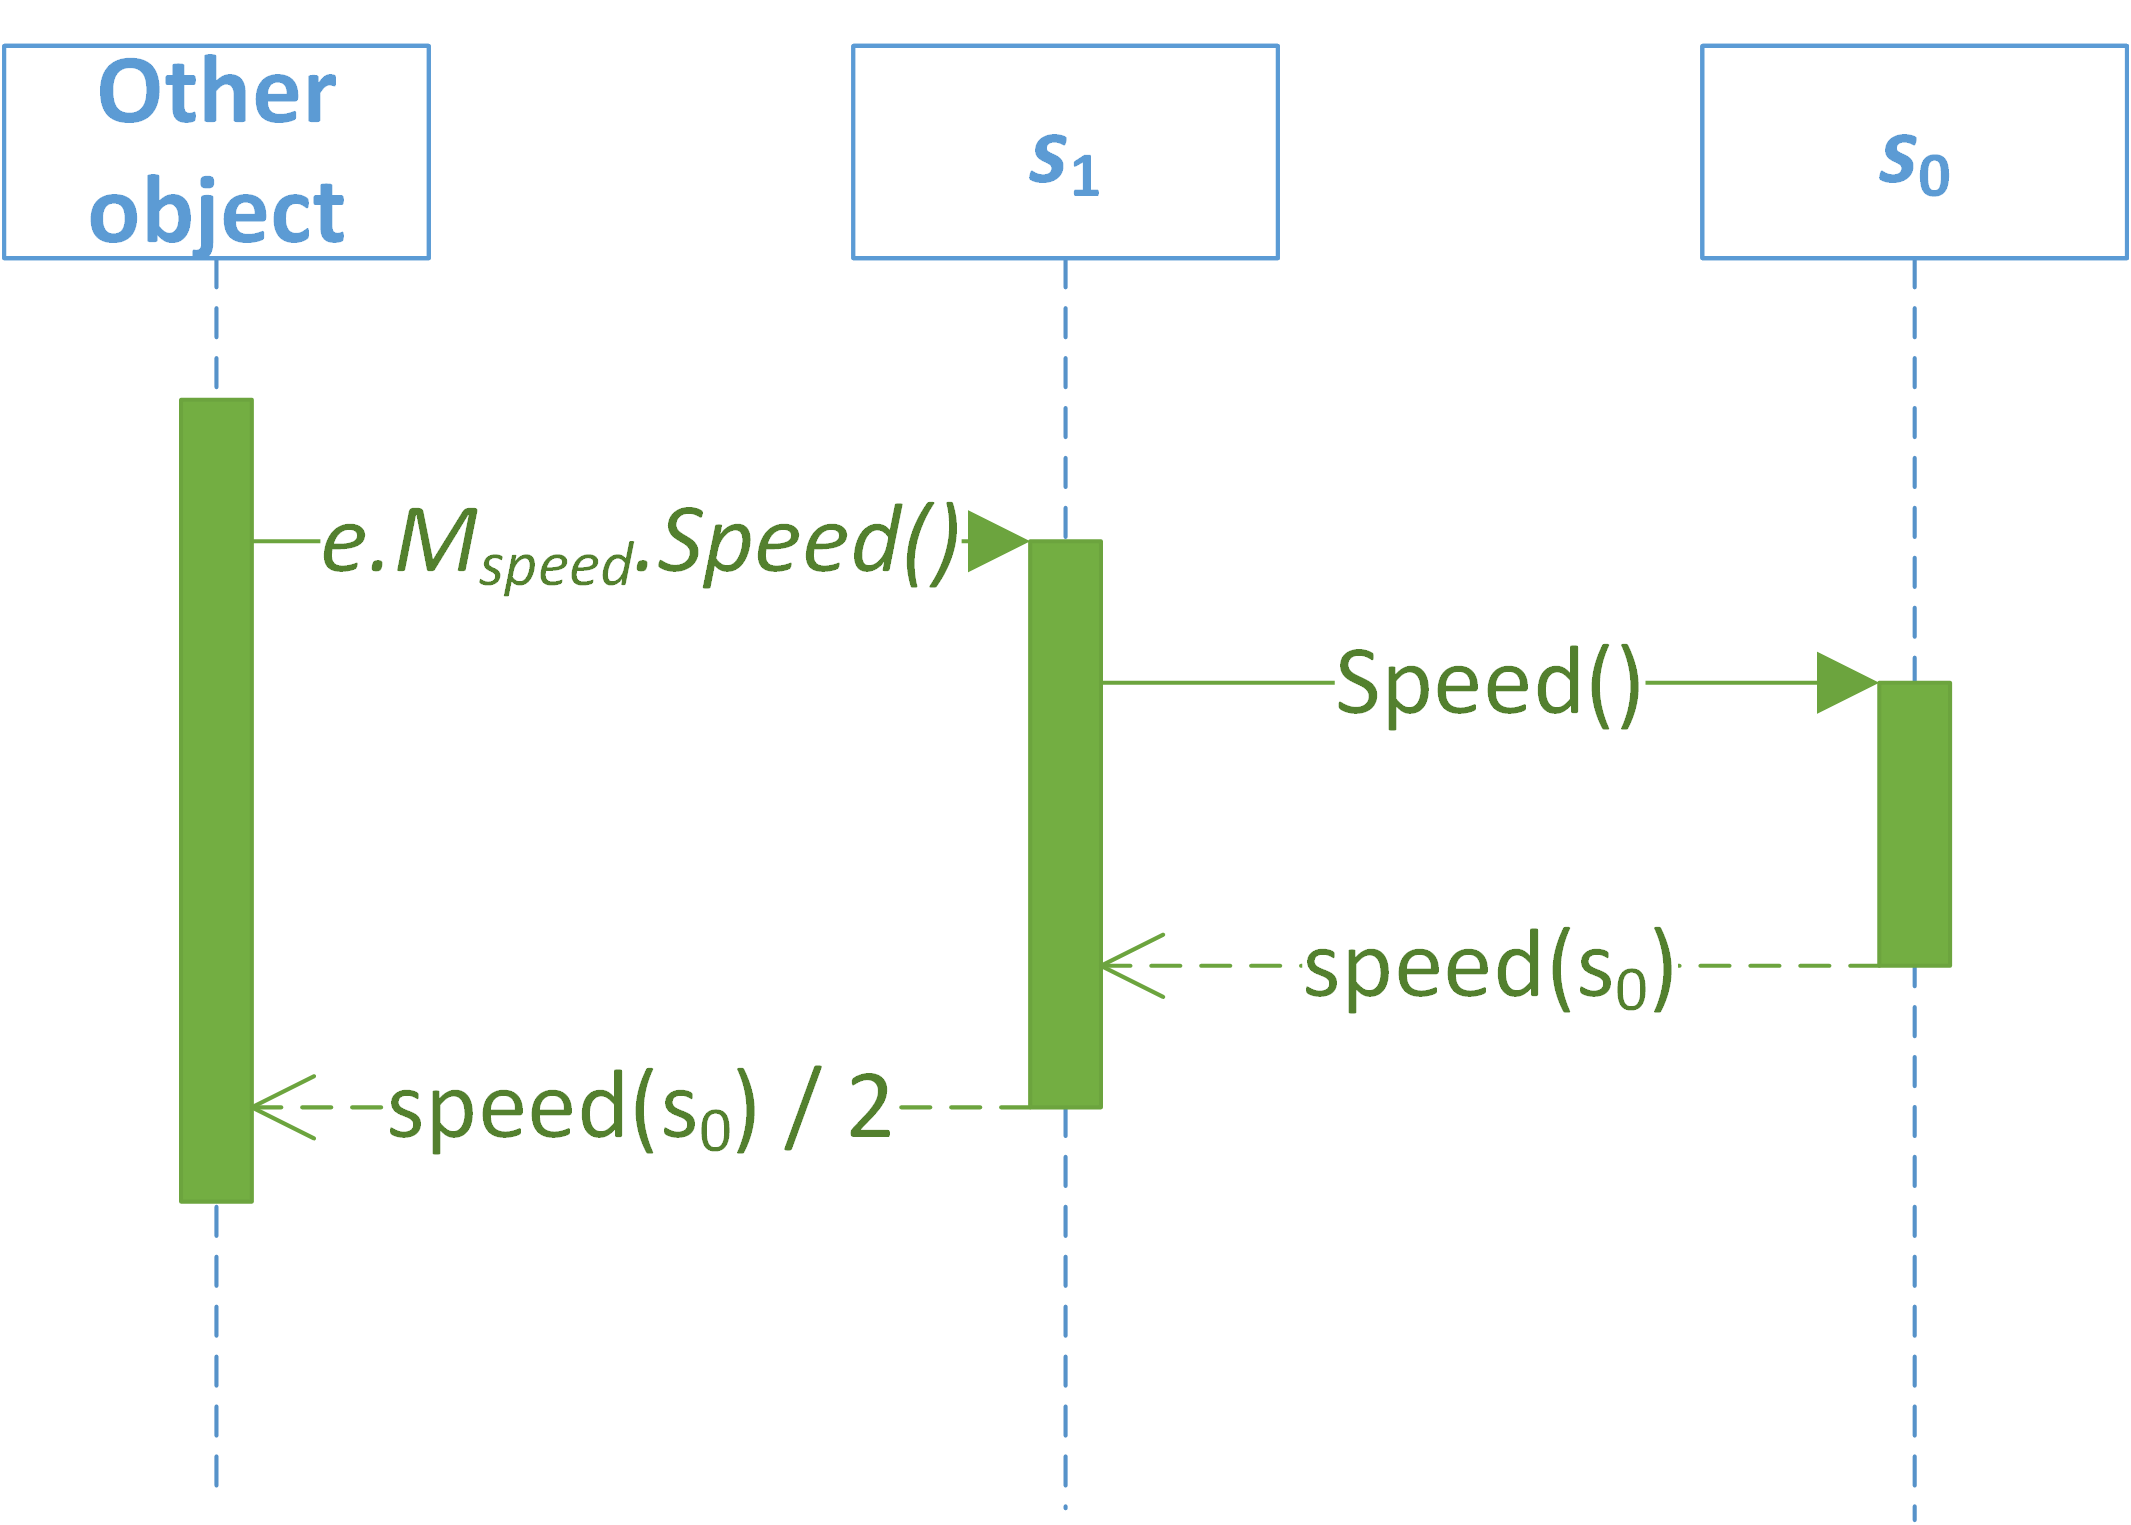
\includegraphics[width=0.6\textwidth]{ModulesChainingExample}
\par\end{centering}

\caption{A \emph{speed} module $s_{1}$ has replaced another ($s_{0}$) of
the same type on entity \emph{e}.\emph{ }Some object requests the
speed of entity $e$ by querying its \emph{speed} module $s_{1}$.
$s_{1}$ then queries the \emph{speed} module it replaced, and returns
half its value.}
\end{figure}


Note that this ``chaining'' of modules can be applied indefinetely,
allowing several modules to affect a single property of the entity.
However, the module methods are called as a stack, which means that
the method of the module inserted last is the first to be called.
This imposes somewhat of a limit, and may not work as desired in all
cases. Consider a stack of $n$ modules, where module $m_{1}$ has
been pushed first, followed by $m_{2}$ and so on, so that $m_{n}$
is at the top of the stack. Then a module $m_{i}$ can not directly
alter the way modules $m_{i+1}\dots m_{n}$ changes it output. This
may or may not be desirable, depending on the situation. It is not
possible, for example, to apply an effect causing an agent's speed
to be set to $x$, no matter what happens, using this method.

Another issue the designer should be aware of is that it is possible
to create a module $m_{1}$ of type $t$, intented to replace another
module $m_{0}$ (as in the above example), and not implementing the
same public methods in $m_{1}$ as in $m_{0}$. Doing this will cause
a runtime exception.

An \emph{agent} is a special entity which have a unique name and can
collect percepts. When an agent is asked to return all of its percepts,
it queries each module for any available percepts, and returns those
as a collection. \texttt{\emph{{[}move this paragraph up (and rewrite?){]}}}



\section{Events and Triggers\label{sec:SystenFeaturesEventAndTriggers}}

In this part the concepts and ideas of both events and triggers will
be explained. We will go through their intention and how to use them
with the engine. Furthermore, a couple of examples will be provided
to give the general idea of what they can be used for. 


\subsection{Concept}

In the natural world, all actions have a reaction, these reactions
could be thought of as events meant to trigger when such actions are
performed. Thus an engine for modeling a virtual environment must
provide as many features as those of the real world environment.


\paragraph*{Events}

To be clear, an event in the context of this engine is the occurrence
of something, for instance an event could be that \textquotedblleft{}an
Agent has moved\textquotedblright{}, or \textquotedblleft{}an Agent
has picked up an item\textquotedblright{}. Furthermore, an event also
has the duty of providing necessary information for the listener,
giving the listener a correct idea of the meaning behind an event.
In the case of the event which signified the movement of an agent,
it is necessary to provide the listener %
\footnote{Listeners refer to the object which is listening to the occurrence
of an event, with the intent of reacting to it%
} with information of which direction the agent moved, where its starting
position is and how far it has moved. Since a listener might be operating
in a different thread, the listener is completely dependent on this
information, as it might no longer be retrievable at the time the
event is being analyzed. For instance, if an agent moved and then
was killed and removed from the world, its position would no longer
be stored in the world. As such, the listener would have no way to
determine where the move had ended if this information was not provided
in the event.


\paragraph*{Triggers}

Triggers in our engine are the means to which listeners gain access
to events. A trigger in our engine is the combination of three different
parts.
\begin{itemize}
\item Events
\item Condition
\item Action\end{itemize}
\begin{description}
\item [{The~events}] are what the trigger is listening for. These can
be any type of event, and a trigger can be registered to any number
of events. But only one event is required to \textquotedblleft{}trigger\textquotedblright{}
a Trigger. For instance, if a Trigger is listening on both the events
\textquotedblleft{}10 seconds passed\textquotedblright{} and \textquotedblleft{}Agent
has moved\textquotedblright{}, then the Trigger will be \textquotedblleft{}triggered\textquotedblright{}
when either of these events occur. However it will be triggered each
and every time such event has occurred and is not limited to just
one occurrence.
\item [{The~Condition}] is a built in predicate for the trigger to check
if it is willing to respond to the event. If the condition is satisfied,
the trigger\textquoteright{}s action is fired. A condition should
only be used in cases that is not covered by another event. For instance,
say you have the event \textquotedblleft{}An agent has moved\textquotedblright{}.
Let us call the agent that moved $a_{m}$ and the agent whose movement
you are interested in $a_{i}$. The condition on the trigger would
then be: 
\[
\textrm{\textbf{is }}a_{m}=a_{i}\textbf{ ?}
\]
\\
As we can see the condition narrows the range of events that are responded
to at the cost of added calculations. In this case it would be much
better to subscribe to the event \textquotedblleft{}Agent $a_{i}$
has moved\textquotedblright{}. This is purely an example as events
can not be tied to specific entity instantiations as events are defined
at compile time.
\item [{The~Action}] of a trigger is the part that performs the work,
it is a method which is executed once an event has been raised and
the condition is satisfied. For instance if a trigger is meant to
write a message when a specific event has occurred, then this is where
the action of writing such a message should be placed.
\end{description}

\subsection{Entities and \texttt{EventManager}}

For triggers to become part of the engine it is required that the
trigger is registered to the engine, however it is of crucial importance
what one registers the trigger to. A trigger can be registered to
either a specific entity or the \texttt{EventManager}. A Trigger registered
to the \texttt{EventManager} will be triggered each time an \texttt{Event}
that it is listening to is fired. However a \texttt{Trigger} registered
to a specific entity will only be informed of events raised on the
specific entity instead of when the event is raised for every single
entity. 

An example of this would be: assume you have a Trigger \texttt{$\mathtt{T_{1}}$}
with the event \textquotedblleft{}An agent has moved\textquotedblright{},
and \texttt{$\mathtt{T_{1}}$} is registered to Agent \texttt{A}.
Additionally, you have a Trigger \texttt{$\mathtt{T_{2}}$} with same
event as \texttt{$\mathtt{T_{1}}$,} but this trigger is registered
to the EventManager. To give a complete picture, also assume there
is an Agent \texttt{B} which has no Triggers registered to it.

This provides us with two scenarios:
\begin{description}
\item [{Agent~\texttt{A}~has~moved:}] In this case, both \texttt{$\mathtt{T_{1}}$}
and \texttt{$\mathtt{T_{2}}$} is triggered, since \texttt{$\mathtt{T_{1}}$}
listens on Agent \texttt{A} and \texttt{$\mathtt{T_{2}}$} listens
on any\texttt{ }agent moving.
\item [{Agent~\texttt{B}~has~moved:}] In this case, only $\mathtt{T_{2}}$
is triggered, for the reasons stated above.
\end{description}

\subsection{Example of making and using an \texttt{Event}}

Let\textquoteright{}s assume one was to make an event which was fired
each time an agent had moved, let us name this Event: \texttt{AgentMoved}.

First, make a class extending the \texttt{XmasEvent} class as shown
below:

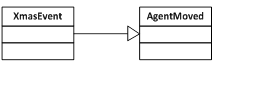
\includegraphics{XmasEventCreationStepOne}

Then, add all the necessary data fields on the newly created event
class.

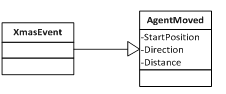
\includegraphics{XmasEventCreationStepTwo}

To utilize the newly created event, it must be raised when appropriate.
In this case, the appropriate place would be to raise it during a
move action.

In this action, after the movement of the agent had been performed,
the method \texttt{RaiseEvent} would need to be called on the entity
that is being moved.


\subsection*{Summary}

Events are what provides the engine flexibility and allows making
reactions to others actions. Events are designed for ease of use and
are meant to be used as much as possible. Triggers are used as a way
to interface with events and they are the only way to connect an object
to the event it wishes to listen to.



\section{Actions}

\texttt{XmasAction}s in the UML Domain model diagram in appendix \ref{sec:Domain-Model-UML}
refers to the object type that performs actions inside the engine.
The reasoning behind these actions being its own class is to ensure
only one action at a time is being performed. This is because there
are many separate threads operating on the model code at once and
as such, there must be a way to active only one action at a time.

For the task of executing the actions we have the \texttt{ActionManager}.
Its job is to take in one action at a time and place them in a queue
(see fig. \ref{fig:ActionQueuing}).

\begin{figure}
\begin{centering}
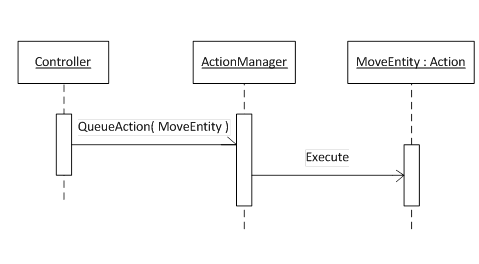
\includegraphics[width=0.7\textwidth]{ActionQueuing}
\par\end{centering}

\caption{\label{fig:ActionQueuing}Sequence diagram illustrating how a \texttt{MoveEntityAction}
is processed. The idea is that a controller, such as keyboard input
or an agent language, queues an action such as moving an entity on
the action manager. The action manager will then execute the action
as soon as it is ready.}
\end{figure}



\subsection{Action Types}

The engine is equipped with two different action types. One of them
is the \texttt{EnvironmentAction}, which are actions that perform
changes on the entire environment. Examples of such actions are closing
this engine or adding/removing entities from the world.

The other action type is the \texttt{EntityAction}. This action type
is meant as an action that a single entity performs; ideally the actions
should be as atomic as possible. In our reference implementation we
have given some ideas how these actions work, such as \texttt{grab},
which is an action that grabs a package from the tile the executing
agent is standing on.


\subsection{Example -- Move Entity Action}

Here we will show how an entity action is constructed by inheriting
the \texttt{EntityAction} class. As shown in fig. \ref{fig:MoveEntityActionExample},
we have created a \texttt{MoveEntityAction} class with one field containing
the direction of the move.

\begin{figure}
\begin{centering}
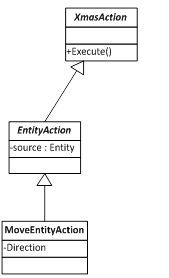
\includegraphics{MoveEntityActionExample}
\par\end{centering}

\caption{\label{fig:MoveEntityActionExample} Illustrating the inheritance
of the newly created \texttt{EntityAction} ``MoveEntityAction''}
\end{figure}


To have the action actually perform something, it is required that
an abstract method \texttt{Execute} is implemented. This execute method
is the method that is executed by the action manager. The implementation
of the execute action could then look something like the following
pseudo code:

\begin{alltt}
\textit{method} Execute \textit{returns} nothing 
    NewPosition = GetPositionOf(World, This.getSource()) + Direction 
    Wait(MOVE_TIME) 
    SetPositionOf(World,This.getSource(), NewPosition) 
\textit{EndMethod}
\end{alltt}

As one can see, the idea is that you find the position of the source
of the \texttt{EntityAction} and use that to generate the new position,
which is its old position incremented by its direction vector. The
wait is there to give the move a speed, as it would otherwise be an
instant movement.


\subsection{Summary}

Using actions is fairly simple and serves to shield the user from
the tedious and error prone workings that takes place behind the scenes.
It is meant to ensure thread safety and allow multiple threads working
with the engine at once. These were the exact reasons we chose this
design, as we ourselves had to deal with the problem of interference
from multiple concurrent threads. Furthermore, it will also reduce
code redundancy as generic actions can be reused by other actions.
The problem with this design is that it in a sense remakes what is
already implemented in a programming language. After all, running
procedural code is what programming languages are meant to do. However,
in return it provides a lot of utility and makes it possible to make
tools for simplifying the process of making actions. It also gives
the ability to differentiate between different action types and even
create new action types if one wishes so.



\subsection{Converting Actions and Percepts}

Both actions and percepts are very abstract objects, and the XMAS
engine can not how they are represented in different APLs. This means
that the system designer needs a way to translate actions from foreign
types into \texttt{XmasAction}s, and \texttt{XmasPercept}s into percepts
of foreign types. We have provided the base necessities for implementing
this functionality with \emph{converters}. A converter is, as the
name implies, a class that takes objects of a foreign type and map
them to internal types or vice versa. \texttt{\emph{{[}Expand{]}}}



\section{Agent Controllers\label{sec:SystemFeaturesAgentControllers}}

The purpose of the agent controllers is to be able to control agents
in the engine from outside. This section will cover our setup of an
agent controller. 

To get an overview of the classes used for the \texttt{AgentController},
look at fig. \ref{fig:AgentControllerDomainModel}.

\begin{figure}
\begin{centering}
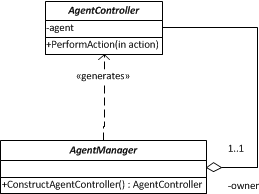
\includegraphics[width=0.7\textwidth]{AgentControllerDomainUML}
\par\end{centering}

\caption{Domain model for Agent Controller\label{fig:AgentControllerDomainModel}}
\end{figure}



\subsection{Concept}

The engine is designed to support the ability to be adapted for all
APL types, this means that the engine itself does not support all
APLs but instead provides a framework for quickly designing interfaces
between the engine and any APL. There are two classes that one must
use in order to properly design the interface:
\begin{description}
\item [{The~\texttt{AgentManager}}] has the duty of speaking directly
with the agent language it attempts to interface with. Its job is
to spawn an \texttt{AgentController} for each agent the AP wishes
to take control of. The \texttt{AgentManager} is in that sense much
akin to an Abstract Factory (see sec. \ref{sec:TheoryFactoryDesignPattern})
, which -- according to the design pattern -- is an abstract class
with a method generating a certain type of object, without restricting
exactly which object is generated, as long as it is of the specified
type. The idea is that if you have a \texttt{GoalAgentManager} then
the controller it constructs would be \texttt{GoalAgentController}.
The methods required by both the \texttt{AgentController} and the
\texttt{AgentManager} are abstract. Thus, we ensure at compile time
that the engine framework is properly used\texttt{\emph{.}}
\item [{The~\texttt{AgentController}}] is the link between a single agent
and the AP. Its job is to take all commands sent to it by the connected
AP, transform them into actions understood by the engine, and apply
them to the agent that it controls.
\end{description}
To simplify the \texttt{AgentController} design, it provides the method
\texttt{PerformAction}, which makes it easy to execute actions on
the agent it controls. When the \texttt{PerformAction} is called,
the \texttt{AgentController} queues the action given through the method
and puts the \texttt{AgentController}\textquoteright{}s thread to
sleep. Once the action has been executed by the engine, the \texttt{AgentController}
is woken up and returns from the \texttt{performAction} method. All
percepts received by the \texttt{AgentController} during this time
is stored on the \texttt{AgentController} and can be easily accessed
by the actual implemenation of the \texttt{AgentController}.

\begin{figure}
\begin{centering}
\includegraphics[width=0.95\textwidth]{AgentManagerAndAgentControllSequenceDiagram}
\par\end{centering}

\caption{This sequence diagram shows the process of an AP taking control of
agent through the \texttt{AgentManager}, and commanding it through
the \texttt{AgentController\label{fig:APConnectingToAndControllingAC}}}
\end{figure}


The process of an AP taking control of an agent is illustrated in
fig. \ref{fig:APConnectingToAndControllingAC}. The AP calls the \texttt{AgentManager}
to locate the agent it wishes to assume control of. The agent is located
through a string (its name) which is unique to it and ensures that
only one agent is taken. When the \texttt{AgentManager} finds the
correct agent, it will immediately generate a new \texttt{AgentController}.
The AP will not gain access to the agent but instead it will gain
access to the \texttt{AgentController}. Now that the AP possesses
the \texttt{AgentController}, it will have the ability to send the
\texttt{AgentController} commands. These commands might not be understood
by the engine if the APL is foreign enough to the engine\textquoteright{}s
own language and as such it is the duty of the \texttt{AgentController}
to convert these commands into actual actions which the engine can
understand.


\subsection{How to use agent controllers}

To use the built-in controller features of the engine, the designer
must provide his own implementations of \texttt{AgentController} and\texttt{
AgentManager}. The designer must do this for every different APL he
wishes to use in the engine.

The classes \texttt{AgentManger} and \texttt{AgentController} both
provides functionality as part of their own classes but also requires
some methods that must be implemented for the classes to function.

For the \texttt{AgentManager }the designer must provide a method that
produces \texttt{AgentControllers} of their implemention, along with
locating an agent though the \texttt{AgentManager} does provide some
assistance in that regard, in the form of a agent locating method
defined as: \texttt{TakeControlOf}, which takes the name of an agent
as a string, and returns the corresponding \texttt{Agent}. Furthermore,
it should be noted that the \texttt{AgentManager} is also automatically
designed to create threads for the \texttt{AgentControllers} it constructs.

For the \texttt{AgentController}, the designer must provide all logic
defining how a controller handles a given agent, this means getting
the percepts from the agent, analyzing the percepts and deciding an
action (Could be outsourced to another APL such as GOAL) and then
queue said action to the agent. The AgentController has the method
\texttt{PerformAction}. This method can be very useful as it queues
an action automatically to its agent, then blocks the thread until
the action has been performed. Furthermore, this action will also
trigger a C\# event called \texttt{PerceptsRecieved} in the case that
the agent controller actually recieve any percepts during the action.
For instance, this event could be used for where the \texttt{AgentController},
decides the next action for the agent to perform, as done in the Vacuum
World Example in appendix \ref{chap:VacuumWorldAppendix}.


\subsection*{Summary}

The agent controller is designed to be very lightweight, since we
do not want to impose any restrictions that might limit an APL which
we know nothing about. As such, the \texttt{AgentController} is more
akin to a convention or a design pattern for how interfacing with
agents should occur. It provides the skeleton of how a link might
be designed but does not impose any restriction on how the link should
be set up.



\section{View}

The engine is designed to assist the user in all parts of the process
when making an environment, this also extends to the visualization
of said environment. However, since our goal is to have as few restrictions
on the model as possible, our knowledge of that view\textquoteright{}s
representation is very limited.


\subsection{Concept}

The view API which the engine provides consists of four abstract classes
that are meant to be implemented by the user. The four classes can
be seen in fig. \ref{fig:ViewUMLView}. We will go through each class
and explain how they are meant to be implemented.

\begin{figure}
\begin{centering}
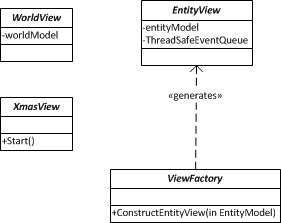
\includegraphics[width=0.4\textwidth]{ViewUmlDomainDiagram}
\par\end{centering}

\caption{UML diagram of the view\label{fig:ViewUMLView}}
\end{figure}

\begin{description}
\item [{\texttt{XmasView}}] The \texttt{XmasView} class is very simple;
it only provides a single method that is required to be implemented.
When the engine starts the view up it generates a thread for the view
and the \texttt{Start} method is the first method to be executed inside
that thread. The start method could contain an endless loop that on
a time interval updates the view. Another task of the implemented
view is also to update its \texttt{ThreadSafeEventManager.} The \texttt{ThreadSafeEventManager}
ensures that events sent from the model thread of the engine is not
immediately executed, but instead lie dormant in the \texttt{ThreadSafeEventManager}
until the view thread is ready to execute them. How many events that
one wishes to execute is up to the user. We also provide the appropriate
methods for the user to specify exactly how long he wishes to wait
for the next event, or if it should timeout. The \texttt{ThreadSafeEventManager}
is very important to the view as without it, designing view code becomes
complicated as one need to constantly ensure that no concurrency bugs
has been applied to the system.
\item [{\texttt{WorldView}}] The \texttt{WorldView} class is added because
of the long term benefits, as of now it provides nothing for the designer.
However if we found benefits to add to the class, making it ahead
of time, even if it is initially empty, can have many benefits as
the project expands.
\item [{\texttt{EntityView}}] Much like the \texttt{WorldView} class, the
\texttt{EntityView} is also very minimal. However, it enforces certain
things that the user of the engine should take care of. First, it
automatically makes a \texttt{ThreadSafeEventQueue} from the entity
and attaches it to the \texttt{ThreadSafeEventManager} which should
be provided by the \texttt{XmasView}. The idea is that all events
the \texttt{XmasView }wishes to listen on should be subscribed to
by registering its triggers on the \texttt{ThreadSafeEventQueue}.
This will ensure that when the view updates the \texttt{ThreadSafeEventManager}
all events pertaining to the specific entity is also updated on the
\texttt{EntityView}\textquoteright{}s triggers, but done so on the
view thread instead of the model thread, separating the two threads
completely.
\item [{\texttt{ViewFactory}}] The \texttt{ViewFactory} is meant to include
all objects with low life cycle used by the view, it is also designed
specifically to construct new \texttt{EntityViews} during runtime
of the engine. In order to know which \texttt{EntityView} belongs
to which \texttt{XmasEntity}, one is required to register all types
of \texttt{XmasEntities} and link it to its counterpart \texttt{EntityView}.
For instance, assume you have a class inheriting \texttt{XmasEntity}
called \texttt{Wall}, and the \texttt{Wall}\textquoteright{}s representation
called \texttt{WallView}, then you need to manually register inside
the \texttt{ViewFactory} that \texttt{Wall} is represented by \texttt{WallView}. 
\end{description}

\subsection*{Summary}

The view framework provides four classes each with their own advantages;
they each represent a part of the model of engine. They are designed
to assist the user in keeping his code threadsafe so that as few problems
as possible arise.



\section{Engine Extensions}

Since most of the engine is very abstract in functionality, we have
made three extensions, which makes it easy to implement a tile based
environment and communicating with EIS.


\subsection{Tile Extension}

This extension represents the world as a two-dimensional array of
tiles using what we will call a tile map. \texttt{\emph{{[}Elaborate
on tile, that entities can move{]}}} We have implemented it so that
the tile in the center has the position $(0,0)$. This means that
all positions are given relative to the origo tile at $(0,0)$. As
a consequence of this, a tile map must have odd dimensions, as it
would otherwise not have a center tile. If the user tries to access
a tile that is out of bounds (for example the tile at position $(0,n+1)$
in a $n\times n$ tile map), a tile containing a special entity signaling
that the tile is not part of the world is returned. This ensures that
querying the tile map for a tile at any position will never fail and
always return a valid value. As well as accessing tiles at arbitrary
positions, the tile map can be queried with a position and a range
$r$, in which case a two dimensional array of size $(2r+1)\times(2r+1)$
is returned, containing the tiles in that square. \texttt{\emph{{[}Explain
that it is relevant in eg. vision. Figure?{]}}}

In the tile extension, we have provided several modules that can be
equipped to agents to make them better suited for inhabiting a tile
based environment. For example, the \emph{movement blocking-} and
\emph{vision blocking} modules apply to all entities with a physical
presence in the environment; given another entity, they specify whether
the entity they are attached to blocks the aforementioned entity's
movement or vision, respectively. The \emph{speed} module defines
how long it takes for the entity to move to an adjacent square. \texttt{\emph{{[}Rewrite{]}}}


\subsubsection*{Vision}

The tile extension also provides means for seeing tiles around an
entity via the \texttt{Vision} module. All entities that are able
to sense their surroundings also have a \texttt{VisionRange} module
which -- as the name implies -- defines how far (in tiles) the entity
can see.

When the vision module is asked to return its percepts, it asks the
world to build it a \texttt{Vision} object, which it returns. The
\texttt{Vision} object uses an algorithm described in appendix \ref{sec:VisionAppendix}
to assemble a set of mappings from positions (relative to the entity)
to tile references. To determine whether a tile $t$ is visible to
an entity $e$, we draw straight lines from each corner of $e$'s
tile to the corners of $t$. If such a line does not intersect with
a tile that is vision blocking with respect to $e$, we say that the
line \emph{connects}. If $e$'s tile has any corner from which we
can connect lines to all corners of $t$, then $t$ is visible to
$e$. If, however, $t$ is itself vision blocking, we require only
two connecting lines, since at least one line would not have to travel
through $t$, and as such not connect.

\texttt{\emph{{[}expand, add image{]}}}

\texttt{\emph{{[}move action, move event{]}}}


\subsection{EIS Extension\label{sub:EIS-Extension}}

The EIS extension provides means for communicating with an EIS instance
over a socket, as well as serializing and deserializing percepts and
actions encoded in an XML representation of EIS' \texttt{iilang} format.
The extension features custom a custom agent controller and manager,
which have been developed to work well with EIS. 

As EIS is implemented in Java and our engine is written in C\#, information
can not easily be passed between the two in a native manner. Instead,
we have opted to have the two communicate over sockets. As EIS already
supports formatting \texttt{iilang} objects to XML, we chose this
to encode information passed over the sockets. We have implemented
our own \texttt{iilang} object tree in C\#, which implements XML serialization
and deserialization (see appendix \ref{sec:iiLang}), as well as a
Java class used to parse XML to \texttt{iilang} objects. Furthermore,
we have implemented special package streaming objects in both C\#
and Java, which sends the size of a payload before the actual data
when streaming XML over sockets\texttt{\emph{{[}Elaborate{]}}}. This
allows us to detect when an XML message has been completely received.
This means that designers wanting to use EIS with our engine should
implement our accompanying Java libraries, as well as the EIS engine
extension.

In order for an EIS instance to connect to an agent controller, it
must connect to a socket which is known by both the EIS instance and
the engine at runtime. The agent manager listens to this socket and
accepts the connection. As the EIS instance connects, it receives
a new socket which can be used to communicate with the agent controller.
It now sends an XML message with the name of the agent on this socket,
and the agent manager constructs an agent controller tied to this
name and socket. The controller and the EIS instance now have their
own private socket connection to communicate on, and the agent manager
proceeds to listen for other APL instances requesting an agent controller.

The EIS instance can now proceed to send actions to be executed to
the agent controller. When such an action is received, the controller
enqueues it, and sleeps till it is finished, at which point it resumes
listening for actions on the socket. The request to return all percepts
is just an action with the name \texttt{getAllPercepts}, which causes
the controller to gather all available percepts from the attached
agent and sent them to the EIS instance via the socket. Note that
by default, this is the only way perepts are sent; percepts are returned
in response to no other actions. Since the agent controller effectively
blocks on actions, the EIS instance can not have the controller queue
other actions or return percepts when it is executing an action that
takes time, such as the tile extension's move action (this is a restriction
imposed by the agent controller base class as described in section
\texttt{\emph{{[}insert section number{]}}}, as it is the default
behaviour of the \texttt{performAction} method). This execution sequence
is very simple, but has some downsides. Consider, for example, that
two agents wish to communicate with each other through the engine
via a \texttt{talk} action. It could be that agent $a_{1}$ wanted
to ask agent $a_{2}$ whether a certain tile was a desirable place
to go. In that case, $a_{1}$'s APL would have the action queued in
the engine, which would execute it and place the question in $a_{2}$'s
mailbox. If, however, $a_{2}$ had just started a lenghty action,
such as moving, its APL would not get notified that it had been asked
a question until the move was complete, and the controller could respond
to the \texttt{getAllPercepts} action. This introduces quite some
delay in performing such actions, which are rather important in a
multi-agent system. 

To remedy this, the system could be designed such that the controller
instead blocked on the call to return all percepts until the agent
had some new percepts available. In the communication example described
above, $a_{2}$ would immediately perceive that $a_{1}$ had asked
it a question, which would cause its controller to send all $a_{2}$'s
percepts (including the question) to the waiting EIS instance. Assuming
that the corresponding AP prioritizes answering the question, $a_{1}$
would have its answer in the shortest possible amount of time. In
general, allowing agents to perform multiple actions at the same time
makes the world more responsible in a number of ways. As another example,
agents in a tile based world (or any world that allows vision) could
subscribe to events on tiles they could see, and be able to respond
when eg. an enemy moved into one of them. This would allow them to
communicate the offenders position to nearby agents, or simply give
the AP a chance to preemptively figure out what the best possible
action would be to execute next. \texttt{\emph{{[}Move to Implementation{]}}}

This method does have some problems. How, for example, does $a_{2}$'s
AP know that it should prioritize answering the question, and not,
say, command the agent to begin a new move action? Since $a_{2}$
is already in the middle of a move, it would most likely break the
rules of the environment. To remedy this, the agents need to return
the action(s) they are currently executing as percepts, and the AP
would have to consider these when choosing actions. For larger environments
and agent programs, this would complicate the agent logic and percept
pool.

\texttt{\emph{{[}Actions and conversion{]}}}


\subsection{EIS and Tile Extension}

\texttt{\emph{{[}Converters and actions for working with EIS in a
tile based environment{]}}}



\chapter{Implementation}


\section{Architecture}

The section will cover how all the components of the engine interacts
with one another, it will detail how flow of information is transferred
through the engine and into the components connected to it. The component
diagram of the Xmas Engine can be found on appendix \ref{ComponentDiagramAppendix}.

The components of the engine are
\begin{itemize}
\item Model
\item World Creation
\item View
\item Controller
\end{itemize}

\subsection{Model Component}
\begin{description}
\item [{Requires:}] \texttt{XmasWorld}, \texttt{XmasAction }and \texttt{Trigger }
\item [{Provides:}] \texttt{Percept}
\end{description}
The model component is responsible for handling internal interactions
of the engine. These interactions are based on which \texttt{XmasAction
}it is given. 

The model component has three requirements, these requirements are
necessary for the model component to properly execute the environment
requested by the user.

The first requirement of the model component is the \texttt{XmasWorld},
the model component uses the \texttt{XmasWorld }by giving it to \texttt{ActionManager},
the \texttt{ActionManager }then gives the \texttt{XmasWorld }to all
\texttt{XmasActions }as they are about to be executed. Thus all \texttt{XmasAction
}executed in the engine use the same \texttt{XmasWorld}.

The second requirement is the \texttt{XmasActions}, all \texttt{XmasActions
}queued on the model component are executed by the \texttt{ActionManager}.
An \texttt{XmasAction }are not executed immediately however as they
wait until all prior \texttt{XmasAction}\textquoteright{}s executions
has been completed. Once queued to the \texttt{ActionManager}, they
are provided with all necessary dependencies such as the \texttt{XmasWorld
}and the \texttt{EventManager}.

\texttt{XmasAction }is designed to allow other threads the ability
to interact with the engine. The reason is that we did not wish for
multiple threads to change the state of the model component at once,
to ensure this was never necessary we provide the abiltity to inject
code into the thread used by the \texttt{ModelComponent}, this code
is transferred in the form of an \texttt{XmasAction}.

The last requirement of the model component is \texttt{Trigger}, the
model component takes any number of triggers and inserts them in the
\texttt{EventManager}. When an \texttt{XmasAction }raise\textquoteright{}s
an \texttt{XmasEvent }on the \texttt{EventManager}, the \texttt{Triggers
}that are registered to that \texttt{XmasEvent }are all triggered. 

The only thing that the model component provides is the \texttt{Percept},
each \texttt{Percept }is something that an agent can sense. An \texttt{AgentController
}connected to the model component can receive these \texttt{Percept}s\texttt{
}which it is meant to use for analyzing the agent\textquoteright{}s
next move.

The model component is made of many classes however the three \texttt{XmasModel},
\texttt{EventManager }and \texttt{ActionManager }are what provide
the core features of the model component and as such is the only ones
shown in the diagram. When going into details of the exact design
of the engine it will be evident that the class \texttt{XmasEntity
}also provides some of the features of both \texttt{EventManager }and
\texttt{ActionManager}, however it only does this to make the feel
of using the engine more natural. For instance when moving an entity
we thought that it would make sense that the code for this was \texttt{Entity.QueueAction(new
Move())}, instead of \texttt{ActionManager.QueueAction(new Move(EntityToBeMoved))}.
In actuality the code does the same thing since in the first case:
All the \texttt{Entity }does is to call the \texttt{ActionManager}
in the same way we just showed and then use itself in place of the
\texttt{EntityToBeMoved}. This is the reason why the \texttt{Entity
}is not shown in the model component as it has no relevance when understanding
the component itself.


\subsection{World Creation Component}
\begin{description}
\item [{Provides:}] \texttt{XmasWorld}
\end{description}
The world creation component is responsible for making a world for
the engine\textquoteright{}s entities to inhabit. The world is created
when the engine starts to execute, as such its internal class \texttt{WorldBuilder
}only contains a blue print for which entities it should construct
and not the actual entities themselves. It does this by storing a
function for each entity, those functions contains the information
on how each of the entities should be constructed.

The user of the engine is meant to implement his own \texttt{WorldBuilder
}class, that implementation should contain knowledge on how the world
he wishes to construct is created. That means if for instance wants
to use a Tile based world then his implementation of \texttt{WorldBuilder}
should construct a tile based world.


\subsection{View Component}
\begin{description}
\item [{Provides:}] \texttt{Trigger}
\end{description}
The view component is meant as the component that visualizes the model
of the engine to the user, it does not enforce how the visualization
is done or in which way the visualization occurs. It only provides
the tools necessary to perform this task.

The view is meant to register \texttt{Triggers }on the model component,
these \texttt{Triggers }contains \texttt{XmasEvents }when an \texttt{XmasEvent
}is raised, the \texttt{Triggers }with those \texttt{XmasEvents }are
triggered. The idea is that when a \texttt{Trigger }is triggered that
means the current state of the model component has changed, the view
uses these \texttt{Triggers }to be informed about such changes, and
are thus able to change its own state in responds correctly making
it able to visualize the new model state. 


\subsection{Controller Component}
\begin{description}
\item [{Requires:}] \texttt{Percept }
\item [{Provides:}] \texttt{XmasAction}
\end{description}
The controller component\textquoteright{}s responsibility is to command
\texttt{Agents }to perform actions inside the world. The controller
component does this by making the \texttt{AgentController }send \texttt{XmasAction
}objects to a specific \texttt{Agent }in the model component. Where
upon that \texttt{Agent }will perform said \texttt{XmasAction}, once
the model component has executed all prior actions.

The controller component also has ability to receive \texttt{Percept
}objects back from the engine, these \texttt{Percept }contain data
about what the \texttt{Agent }it is controlling has sensed. These
\texttt{Percepts }are meant to be analyzed by the controller component
to determine what its next \texttt{XmasAction }should be. 

The controller component is made up of abstract classes which the
user of the engine must first implement; these implementations could
be setup to act as an interface between a single APL and our engine.
This means that for each APL one must make a new implementation of
the controller component. To reduce the burden of the user we will
in our extensions provide the ability to interface with EIS supported
APLs.

Furthermore the controller component is not only designed to make
interfacing with different APLs easier, it is also meant to be used
when making an interface between the user and the model component.
For instance if one wished to control an agent with the keyboard,
then an Keyboard implementation of the AgentController and AgentManager
should be made, where it would be possible to bind the queuing of
move actions to specific buttons on the keyboard. 


\subsection*{Summary}

The architecture of the engine shows the connectivity between each
of the components. The Model component which job it is to ensure proper
interactions occur inside the world. The world which is constructed
by the World Creation Component, meant to be designed along with the
world itself. 

The interactions of the model component are provides by the controller
component which task it is to command the agents inside the engine,
and make it so they are given intelligence. And lastly the view component
which only task is to visualize the state of the engine.



\section{Model}


\subsection{World}

To be able to unambiguously reference an entity, they are assigned
an \texttt{id} (represented as a number) in the engine. This is relevant
when, for example, a backend APL such as GOAL executes an action involving
other entities than the agent it is controlling. In this case, the
entity's position can be amiguous, since several agents may very well
occupy the same spot in the world.

To hold references to all entities in the environment, the \texttt{XmasWorld}
class contains a set of mappings (a C\# \texttt{Dictionary}) from
\texttt{id}s to entities. Since all agents have a name, it also contains
mappings from names to agents. 

When an entity is added to the world, the variable holding the last
used \texttt{id} is increased by one, and the entity is associated
with this number. This ensures unambiguity, since no number can be
used twice. However, it does impose a limit on the number of entities
that can be added to the world. We have represented the \texttt{id}
as a 64 bit unsigned integer (C\#\texttt{ ulong} type), so it supports
adding more than $1.8\times10^{19}$ entities. In an environment that
is meant to run indefinetely, and where entities are added and removed
often (such as a server based website indexing tool), this limit may
be a concern. 

The process of assigning \texttt{id}s to entities is handled in the
\texttt{AddEntity} method, which takes as arguments the entity to
be added and an \texttt{EntitySpawnInformation }object, containing
the desired position of the entity in the world, and any other relevant
information, such as initial state. However, this only occurs after
the user-implemented method \texttt{OnAddEntity} is called with the
entity and spawn information as arguments, and has returned success.
This method is overridable by the designer, and can be used to ensure
that entities are added properly to the custom world, or not at all.
For example, if the world has the restriction that no two entitites
can start in the same position, \texttt{OnAddEntity} can be implemented
so as to return failure when an the entity in question would be spawned
in an occupied position. Alternatively, it may correct the error,
for example by placing the entity in an adjacent, unoccupied square
and return success. In any case, the \texttt{AddEntity} method propagates
the return value from \texttt{OnAddEntity} to its caller when it returns.

The \texttt{RemoveEntity} method dereferences the entity by removing
itself and its \texttt{id} from the previously mentioned set of mappings.
Similarly to the \texttt{AddEntity} method, it calls the user-supplied
\texttt{OnRemoveEntity} method, and returns its return value. 


\subsection{Entities and Entity Modules}

When designing the \texttt{Entity} class, we wanted to detach the
properties and behaviour of entities from the class itself, and segmentize
them into smaller, succinct objects. In essence, we wanted to be able
to construct an entity that could, for example, move and speak by
assembling it from a movement object and a speaking object. In object
oriented programming languages such as C\#, problems like this are
typically accomplished by means of inheritance. It would indeed make
sense to let a \texttt{MovingAndSpeakingAgent} class inherit from
the \texttt{MovingAgent} and \texttt{SpeakingAgent} classes, which
would then provide the desired behaviour. Unfortunately, C\# does
not support multiple inheritance; a class can not directly inherit
from more than one class, although it can inherit multiple interfaces.
Instead of using inheritance, we designed the module system described
in section \ref{sub:SysFeatEntities}.


\subsection{Events and Triggers\label{sub:ImplementationEventsTriggers}}

This section will cover the inner workings of how events and triggers
are connected, as well as detail why we designed it the way we did.
We will also cover the exact procedure when an event is raised, to
defuse any confusion there might be as to what happens inside the
engine.


\subsubsection*{Explanation}

By themselves, events are not particularly complicated since they
are essentially just data structures that are transferred to all its
listeners upon triggering. As such we shall do a close examination
of how exactly the\texttt{ EventManager }works.

The \texttt{EventManager} is tethered through the engine to all entities
that are inside. Whenever an entity has an event raised on it, it
is copied to the event manager which also raises the event. The intent
is to minimize the number of events needed to cover a single case.
To be clear on how exactly this transpires, we have drawn a sequence
diagram.

\texttt{\emph{}}
\begin{figure}
\begin{centering}
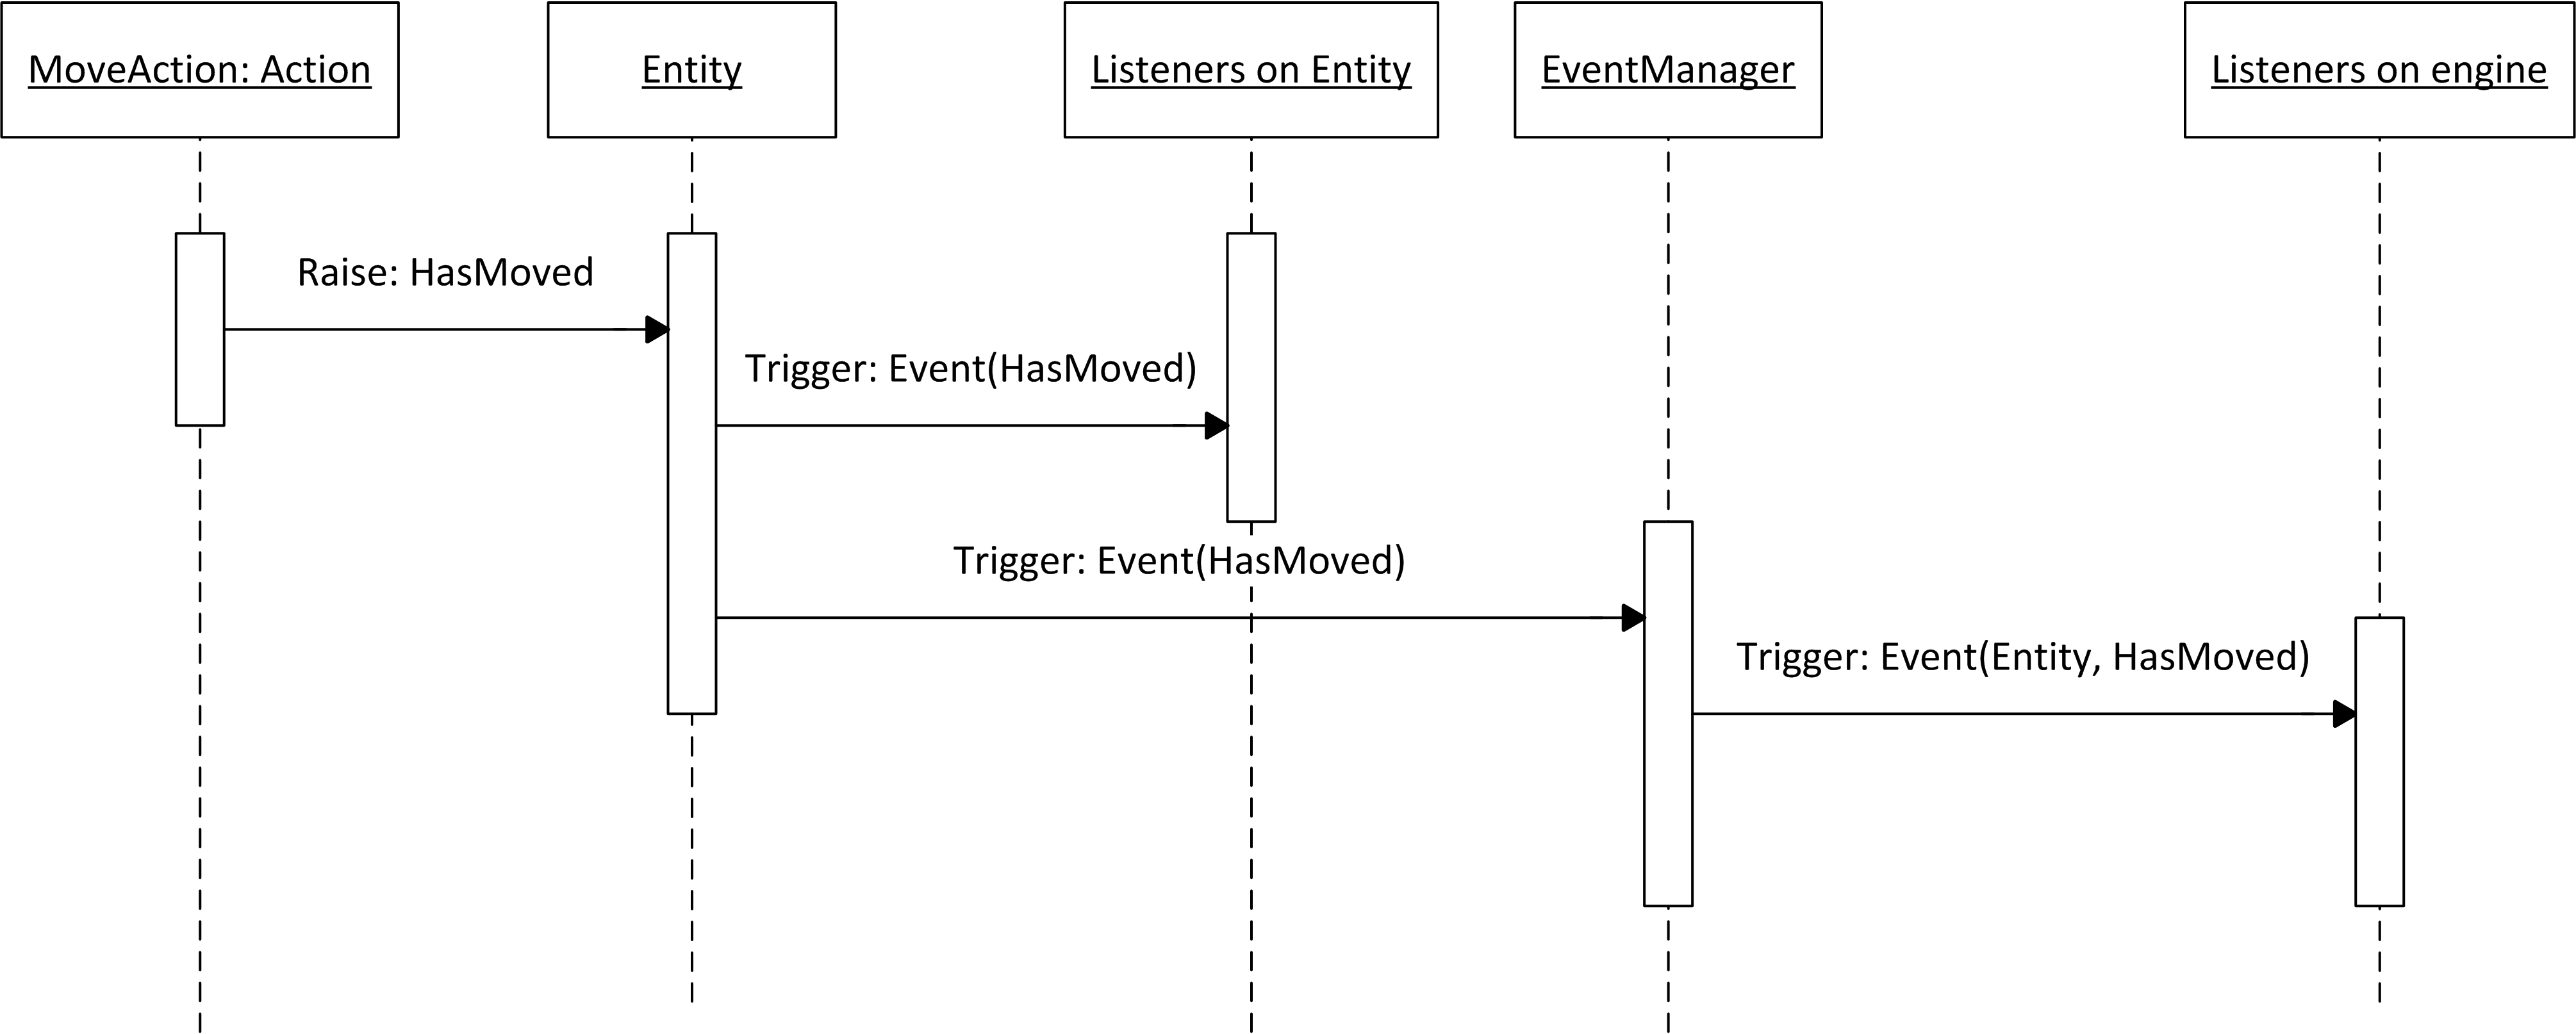
\includegraphics[width=0.7\textwidth]{ImplementationEventAndEventManagerSequenceDiagram}
\par\end{centering}

\texttt{\emph{\caption{\texttt{\emph{A sequence diagram of an event being raised on an entity\label{fig:ImplementationEventAndEventManagerSequenceDiagram}}}}
}}

\end{figure}


As shown on fig. \ref{fig:ImplementationEventAndEventManagerSequenceDiagram},
an action -- in this case a move action -- raises an \texttt{EntityMovedEvent}
on a given entity. The entity then calls all triggers registered to
it, where the trigger also contain the event being raised. After this,
the entity informs the \texttt{EventManager} that an event has been
raised on it, which causes the \texttt{EventManager} to also call
all its registered Triggers with the given Event. Once all relevant
triggers have been informed of the Event being raised, the procedure
is complete and the \texttt{EventManager} returns to its dormant state.

In the case of events that are not linkable to a specific entity such
as an \textquotedblleft{}Engine Close Event\textquotedblright{}, the
event is raised purely on the \texttt{EventManager} itself. Otherwise,
the process is exactly the same as above, except that no particular
entity is involved.


\subsubsection*{Considerations}

As there were many considerations that went through our design process,
we will take each component of this area and break down why exactly
why we designed it as we did.


\paragraph*{Problems of C\# events and why we chose to design our own events}

The language which our engine is written in is C\#, one of the good
things about C\# is that events is built into the language. As such
it may come as a surprise that we have chosen to re-implement events
ourselves. However, while the name might be the same, the intent between
C\# events and our events is so different that it is impossible to
compare the two. The intent behind C\# events is to keep maintenance
on single objects, so that changes to a given object can affect its
linked objects without having to be designed specifically to do so.
This allows for really decoupled projects and is what makes object
maintenance in C\# easy. However our events are not meant for such
low-level tasks. Instead they are meant to allow reactions to occur
in response to other actions. Furthermore, C\# actions are bound to
a specific class, and can only be fired inside methods of an instantiation
of the specific class. The events we have designed are meant to be
raised by all types of class that wish to signal such an event has
occurred.

To give an idea of what sort of problems that would arise from using
C\# events, one need only look at how global events would have to
be implemented. Since Events using C\# are linked to a specific class,
this would essentially mean that the EventManager class would need
to be setup for every single event the engine is capable of running.
What this basically has accomplished is to couple a single class into
the entire workings of an engine, this makes the engine difficult
to extend and modify at a later time since the design would be practically
hardcoded into it. 


\paragraph*{Improvements of events}

As of now, our events are not tied to being \texttt{EntityEvent}s
or \texttt{EnvironmentEvent}s like actions are, however this might
have been a wrong move on our part. The problem is that the user of
the engine might be unclear as to which is what, currently the difference
lies in the name convention used for events. For instance, it is clear
from the name that the \texttt{EntityMovedEvent} can be tied to a
specific entity. In the case of the \texttt{AddedEntityToEngineEvent},
however, there is some ambiguity, as the event is clearly speaking
about a single entity, but as the entity is only just added it would
have been impossible for any trigger to be registered to it. If one
was to make improvements to the event design this would be one change
that was worth looking into.


\paragraph*{Triggers}

The trigger design came about as a necessity for providing a way for
the user to easily design reactions to a given event. The trigger
design is very minimalistic except for the fact that it has a condition.
We designed it with the condition because we wanted it to be obvious
how unwanted events should be handled. Furthermore it also helps to
split up the code containing if the action should be executed away
from the action itself allowing for more readable code. 

Another way the triggers could have been designed would be if the
user simply registered lambda functions (anonymous function), this
would help reduce the amount of classes a user should know and understand.
However we preferred to encapsulate this into what we call the Trigger,
since we wanted to have the ability to expand the capability of the
trigger at a later time.

In short, triggers are a simple design that gives the engine user
a lot of flexibility. 


\subsubsection*{Summary}

Events and triggers might be a hassle to setup and design, but in
return they provide the engine with a lot of flexibility. Without
Events the engine would suffer greatly and all actions would be required
to be bogged down with a lot of extra logic. This would not only remove
the modularity of the engine but also make using the engine more error-prone.


\subsection{Actions}

As we already went through what actions can be used for, this section
will instead focus on the idea behind actions, and how we implemented
them. It will furthermore cover the entire life span of an action
object.


\subsubsection*{Explanation}

An action -- or \texttt{XmasAction,} as it is called in our engine\texttt{
}-- is a class which provides an API for performing state changes
inside the engine, while also ensuring that only one action at a time
is being executed. 

\begin{figure}
\begin{centering}
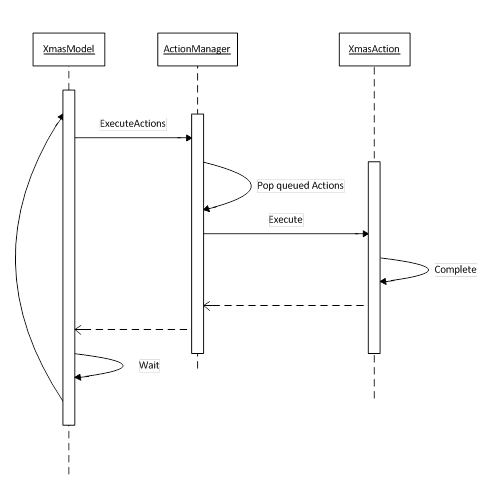
\includegraphics[width=0.7\textwidth]{ImplementationActionQueuingExplanation}
\par\end{centering}

\caption{\label{fig:ImplementationActionQueuingExplanation}A sequence diagram
describing the execution of an action.}
\end{figure}


As can be seen in fig. \ref{fig:ImplementationActionQueuingExplanation}
it starts with the \texttt{XmasModel} running an endless loop that
tells the \texttt{ActionManager} to execute all newly queued actions.
The \texttt{ActionManager} then takes all the actions from a thread
safe list and places them in a local list. After this, each action
is executed individually, putting the action that is being executed
in a running state, this state will not change before the actions
\texttt{Completed} method is called. Once an action has been properly
executed, it will be changed to a completed state and will be properly
disposed of. When the last action has been executed by the \texttt{ActionManager},
the call to \texttt{ExecuteActions} returns and \texttt{XmasModel}
will put the thread in a waiting state. The \texttt{XmasModel} will
remain in a waiting state until a new action has been placed on the
queue; this prevents it from busy waiting when no actions are to be
executed.


\subsubsection*{Considerations}

The way that action completion is designed might seem tedious in that
it has to call the special method \texttt{Completed} on each action.
However it is quite necessary as the completion of the execute method
call does not guarantee that a method is completed, for instance in
the case of non-instantanious actions, as explained in the example
below. 

Consider the action of moving from one place to another. In this case
the move action would need to set a delay before the actual move,
to give the idea that the move action had a speed. As we can\textquoteright{}t
halt other actions during this time it is paramount that the \texttt{Execute}
method is released so that other actions can be executed during this
period. 

This is also how the move action is designed in our reference implementation,
the algorithm is as follows
\begin{enumerate}
\item The move action is put on the queue 
\item The move action sets up a timer on a different thread and finishes
its execution
\item The timer is fired after a given time, and places a new action on
the queue
\item The new action performs the actual move, and calls the \texttt{Completed}
method of its parent Action (the \texttt{MoveAction})
\end{enumerate}
As one can see, the problem in this design is the redundancy created
by having to call the method \texttt{Completed }on every designed
action execution. This might not seem like a problem but it is problematic
in a few ways. First and foremost it adds complexity in usage of the
engine, a person with no knowledge of using the engine would not intuitively
deduce the correct way to make and use actions. Thus it creates a
second problem: there is no way to determine if an action is correctly
constructed during compile time. This means bugs will naturally accumulate
during extended use, even if a user has experience and foreknowledge
forgetting even for a single action can be crucial. This is because
running actions use resources and if never completed the resources
of the actions are never released. For instance let us assume the
\texttt{MoveAction} \texttt{Completed} method is never called, the
result of this is that it is stored in the \texttt{ActionManager}
as \texttt{Running}. Now let us assume that this move action is continuously
being executed by hundreds if not thousands of agents. As each action
is never released the memory stored for each action is never released
and an unintentional memory leak is thus created.

Another way we could have chosen to implement the action completion
process, is the usage of child action. Imagine if an action could
generate new actions that were linked with it, thus the completion
of an action would be tied to the fact that all its child actions
had been executed and not the arbitrary call of a \texttt{Complete}
method. This could undoubtedly provide new problems to overcome and
as such we have not fully followed this path, however given more time
to study the consequences of this design would reveal whether or not
this is a better design. 


\subsubsection*{Summary}

A lot of the considerations when designing the action all comes down
to the reliance on user to clean up the Action, which is generally
not good from a design perspective; it is always preferable that used
data is cleaned up automatically when it is out of scope. However
it is not all bad as this design does guarantee a flexible usage of
the actions; it provides more control to the user which might give
the user abilities to do certain things which would otherwise be denied
within the engine. This is also why this design method was chosen
as our philosophy in the engine design was to minimize limitations
as much as possible while still providing the features we thought
necessary to fulfill the engine's goal.



\subsection{Agent Controller}

The agent controller is designed specifically to be able to accommodate
all types of APL. This means that a lot of special care had to be
taken in order for us to impose as few restrictions as possible. This
section will focus on the different designs we went through and why
we eventually landed on the design we have now.

\begin{figure}
\begin{centering}
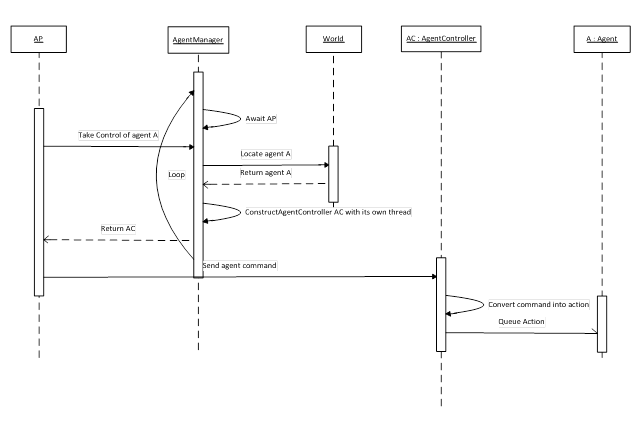
\includegraphics[width=0.7\textwidth]{ImplementationAgentControllerSequenceDiagram}
\par\end{centering}

\caption{This image details exactly how an \texttt{AgentManager} Processes
incoming requests from an outside AP \label{fig:ImplementationAgentControllerSequenceDiagram}}
\end{figure}



\subsubsection*{Explanation}

The \texttt{AgentManager} is designed to run separately from the engine\textquoteright{}s
model thread, which means it has the ability to take all the time
needed to properly connect to an outside AP, same goes for the \texttt{AgentController}.
This means that when an \texttt{AgentManager} generates a new \texttt{AgentController}
to be used by the AP, it also generates a new thread which the \texttt{AgentController}
is executed on. In the System Features section we covered how \texttt{AgentController}s
are used. Here we will elaborate on the exact process. In fig. \ref{fig:ImplementationAgentControllerSequenceDiagram},
a sequence diagram is shown that looks familiar to the one shown in
the system features. However there are a few key differences. First,
this sequence diagram shows the complete life cycle of an \texttt{AgentManager},
since the \texttt{AgentManager} is running on its own thread it does
not care about blocking until work needs to be done and the only kind
of work it is responsible for is ensure that \texttt{AgentController}s
are generated for APs in need of them. Second, it also details that
\texttt{AgentController}s are in fact generated by the \texttt{AgentManager}
with its own thread.


\subsubsection*{Considerations}

The \texttt{AgentManager} went through many design iterations in order
to arrive at its present state. Originally, the \texttt{AgentManager}
was called \texttt{AgentServer}. The reason was that for another language
to interface with the language of the engine -- C\# -- there must
be a universal way of connecting the two languages. A way in which
practically no languages was prohibited from interacting, and as we
thought such a way could only be achieved through a TCP connecting
since the protocol for TPC connections is very old and as such usable
in most languages by far. While it is true that probably almost all
languages do require a TCP connecting in order for them to work with
our engine, it is not true for languages that the engine understand,
considering that all the .NET platform languages works together very
well. For example, you could use the functional programming language
F\#, which also runs on the .NET platform. As such, if we imposed
that all \texttt{AgentManager}s are \texttt{AgentServer}s, it would
be required to setup a server just for using a language which the
engine already understands. \texttt{\emph{{[}Consider rewriting paragraph
from another standpoint: AgentManager is more general, less restrictive
than AgentServer{]}}}


\subsubsection*{Summary}

\texttt{AgentManager} and \texttt{AgentController} is designed as
a framework for making an interface between an APL and the engine.
They are intentionally made very lightweight so that they do not prohibit
the any special requirements of any given APL.



\section{View}

As the view our engine provides is only a framework for making an
actual view, it limits what can be said about its implementation.
What this section will focus on is why we chose to design the view
in this manner and how we provide ways to ensure that the view can
be executed on a different thread while not being affected by its
problems.

\begin{figure}
\begin{centering}
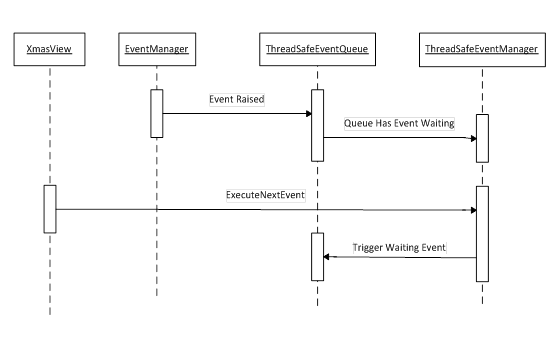
\includegraphics[width=0.7\textwidth]{ViewImpThreadSafeSequenceDiagram}
\par\end{centering}

\caption{Sequence diagram show how events triggered on the model is stored
and put on hold until the view thread is able to process them\label{fig:ThreadSafeSequenceDiagram}}
\end{figure}



\subsection*{Design}

The view design for the engine was never meant to be an actual view,
this would limit the potential of what could be done so we are rather
content with not providing more than the skeleton for making a proper
view. The idea is that the actual implementation of a view should
be part of some extension to make a view that displays graphics or
a view that shows a console, it should never be a core part of the
engine. The core engine should only provide what all views need, this
means that if just a single view is restricted by our design then
our design is flawed.


\subsection*{Thread Safety}

One thing all views have in common is the dangers of having code that
is not thread safe, by having two threads run through the same address
space at the same time, the guarantee of a race condition or deadlock
is very high. This makes programming a view rather difficult. To combat
this problem, we came up with the \texttt{ThreadSafeEventManager}
and the \texttt{ThreadSafeEventQueue}. These classes both assist with
ensuring that the model thread is never involved in the view thread\textquoteright{}s
business. The way the \texttt{ThreadSafeEventManager} works is by
storing all events triggered by the EventManager of the model, the
events data are all kept safe and the order in which the events was
triggered is also kept. The idea is that when the view thread is not
performing any actions, such as when it is in sleep mode between a
draw update, instead of sleeping it will call the \texttt{ThreadSafeEventManager}
and tell it to begin executing. The process works by running the \texttt{ThreadSafeEventQueue}
that had one of its events trigger and tell it to execute. When all
\texttt{ThreadSafeEventQueue} are empty then that mean that there
are no longer any events waiting to be executed on the view thread.
Since views are only interested in seeing the changes to the world
and not how the changes came about, then that means that the views
only need access to the events and not the actions. To see a sequence
diagram of this process look at fig. \ref{fig:ThreadSafeSequenceDiagram}.


\subsection*{Summary}

The view design is mostly focused on ensuring that the user of the
engine should deal with as few threading problems as possible as such
we have developed two classes \texttt{ThreadSafeEventQueue} and \texttt{ThreadSafeEventManager}
these both make it possible for the view to trigger events when the
thread is free from other duties, instead of relying on the model
thread to also handle view event updates. 



\section{Engine Extensions}


\subsection{Tile Extension\label{sub:ImplementationTileExtension}}


\subsubsection*{Vision}

As the basic rules for which tiles can be seen from where have been
explained in the System Features section, we will now turn our attention
to how corners are connected with each other. 

\begin{figure}
\begin{centering}
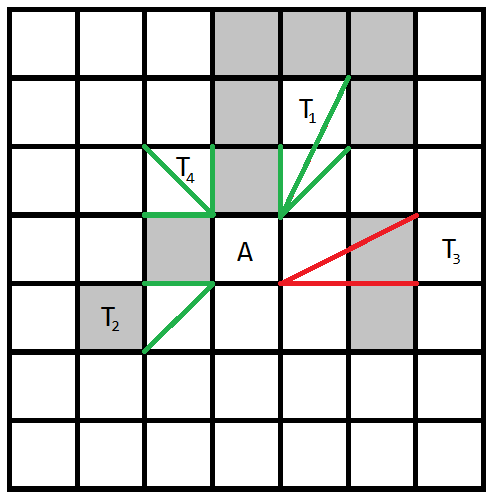
\includegraphics[width=0.5\textwidth]{tilemapVision}
\par\end{centering}

\caption{In this figure we see the visibility of selected tiles $\mathtt{T}_{1}\dots\mathtt{T}_{4}$with
regards to the agent in position $\mathtt{A}$. The light gray squares
represent vision blocking tiles, and all other tiles are see-through.
Lines have been drawn from the corners of the agent's tile to the
corners of the selected tiles. Green lines signifies that the two
corners connect, whereas red lines means they are not connected. Tiles
$\mathtt{T}_{1}$, $\mathtt{T}_{2}$ and $\mathtt{T}_{4}$ are visible
to the agent, while $\mathtt{T}_{3}$ is obscured.\label{fig:TileMapVision}}


\end{figure}


We say that a corner $c_{1}$ on a tile $t_{1}$ connects to a corner
$c_{2}$ of another tile $t_{2}$ if a straight line can be traced
from $c_{1}$ to $c_{2}$ without intersecting with a tile that is
blocking the line. In the tile extension, a tile is blocking the line
if it contains an entity that is vision blocking with respect to the
entity looking from $t_{1}$. This presents a problem with a line
whose vector has an $x$ or $y$ component equal to 0. As such a line
never intersects with any tiles (it only passes between them), it
will always connect with the rules stated above, even if all tiles
it passes are vision blocking. Thus, we say that a line which only
extends in the $x$ or $y$ direction does not connect if it passes
between two vision blocking tiles.

Recall that the tile $t_{2}$ is visible from $t_{1}$ if at least
one corner of $t_{1}$ connects to at least three corners of $t_{2}$.
If $t_{2}$ is vision blocking, only two corners of $t_{2}$ need
be connected to. In figure \ref{fig:TileMapVision} we have shown
some examples of connecting corners. Note that the line from the SE
corner of \texttt{A} to the SW corner of $\mathtt{T}_{3}$ does not
connect, as it passes between two vision blocking tiles, as described
above. Also note that $\mathtt{T}_{4}$ should, intuitively, be obscured
to the agent; we should have a rule saying that when a line intersects
with a corner, it should be blocked if both of the two tiles that
are connected to the corner, and is not intersected by the line, are
vision blocking.

In its most simple form, the vision algorithm iterates over all the
tiles in the agent's visible range, and returns a collection containing
just those satisfying the above condition, as shown in the pseudo
code below:

\begin{alltt}
\textit{Method} Vision 
        \textit{takes} an Agent A, 
        \textit{returns} a collection of Tiles
    Tiles : Collection of Tiles
    for each Tile T in A's visible range:
        \textit{if} T.isVisionBlocking(A):
            \textit{if} any one corner of A connects with any two corners of T:
                add T to Tiles
        \textit{else}:
            \textit{if} any one corner of A connects with any three corners of T:
                add T to Tiles
    \textit{return} T
\end{alltt}

\begin{figure}
\begin{centering}
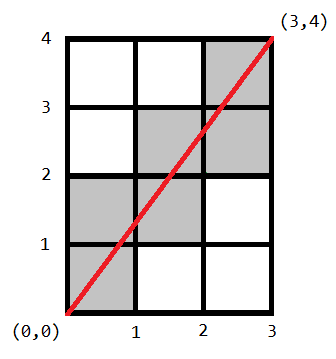
\includegraphics[width=0.4\textwidth]{tilemapConnection}
\par\end{centering}

\caption{A line described by the vector $v=(3,4)$ with slope $s=\frac{v_{y}}{v_{x}}=\frac{4}{3}$.
Squares in light gray are tiles the line intersect with.\label{fig:ConnectingLine}}
\end{figure}


The interesting part of the algorithm is this: how do we determine
whether two corners connect? That is, how do we find all the tiles
a line from one corner to another passes through? To illustrate the
problem, consider the line depicted in fig. \ref{fig:ConnectingLine}.
First, we find the slope of the line as $s=\frac{v_{y}}{v_{x}}$,
where $v$ is the vector describing the line. If we consider the line's
equation ($y=s\cdot x$), as it is depicted in the figure, we can
see that the line segment decribed by the vector between the points
$\left(x_{0},s\cdot x_{0}\right)$ and $\left(x_{0}+1,s\cdot\left(x_{0}+1\right)\right)$
(where $x_{0}\in\mathbb{N}$) crosses the tiles between $x=x_{0}$
and $x=x_{0}+1$ on the $x$-axis and $y=\left\lfloor s\cdot x_{0}\right\rfloor $
and $y=\left\lceil s\cdot\left(x_{0}+1\right)\right\rceil $ on the
$y$ axis. This can be repeated for every $x_{0}$ in the range $0\dots v_{x}$
to obtain the complete collection of intersected tiles.

Additional complications occur when $v$ has negative components,
or when $v_{x}$ or $v_{y}$ is zero, but this outlines the basic
principle of the algorithm.


\subsection{EIS Extension}

EIS support to the engine to the engine is provided with a special
\texttt{AgentController/AgentManager }class, along with a specially
designed java EIS environment jar file. This section will go through
how the implementation works and how we connect to the EIS environment.

The EIS environment in java and the agent controller on the engine
is connected through a TCP connection. They commicate with each other
with XML as a markup language for the data they transmit. 

Fig. \ref{fig:DeploymentEISandAgentController} shows the setup between
EIS and the agent controller.

\begin{figure}
\begin{centering}
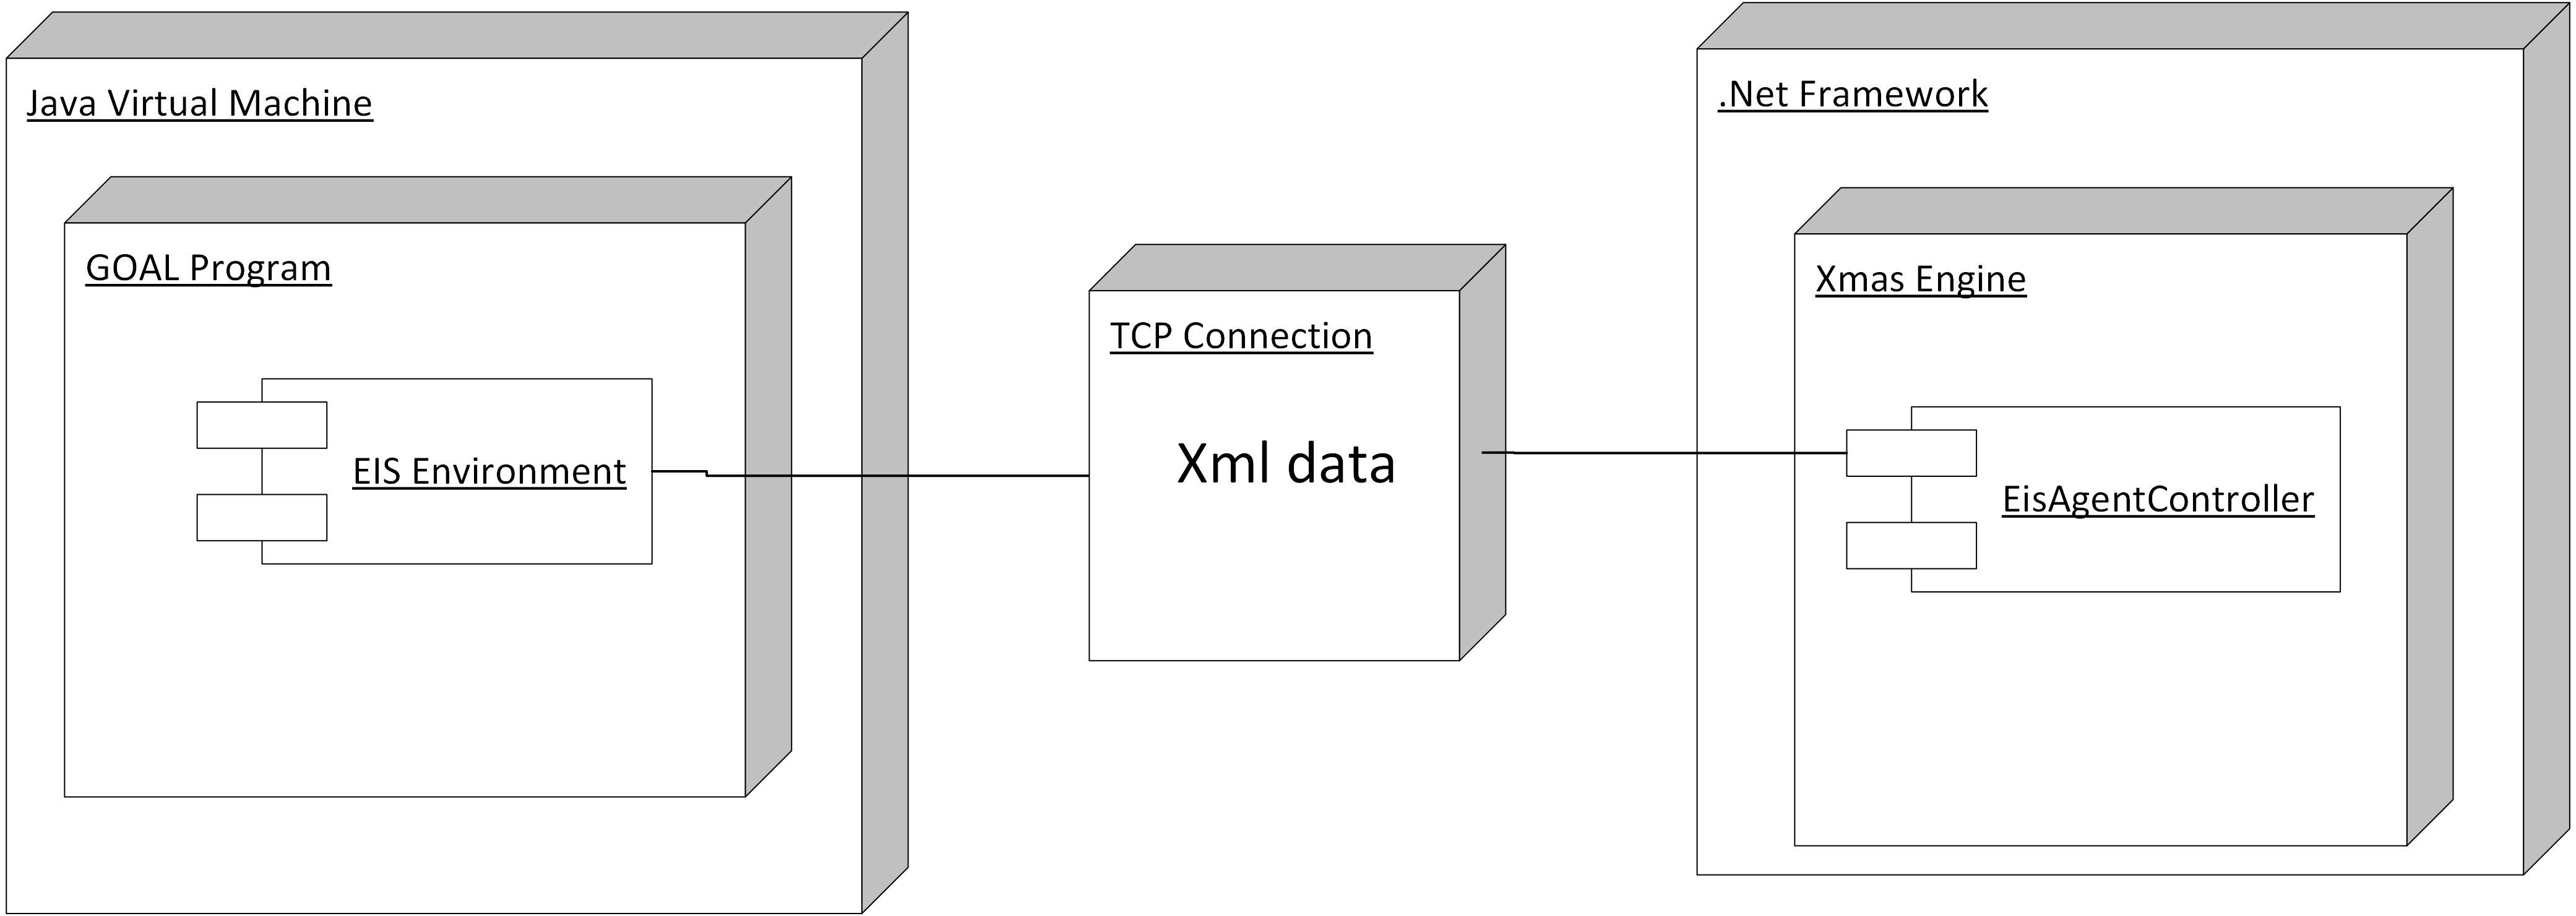
\includegraphics[width=1\textwidth]{DeploymentEISandAgentController}
\par\end{centering}

\caption{An illustration of the connection between the EIS environment and
the agent controller.\label{fig:DeploymentEISandAgentController}}


\end{figure}


Although the EIS environment and the agent controller sends all data
in form of XML data there is one difference and that is all XML nodes
are packaged into packages of a certain size and the size is sent
before the xml data, as can be seen in fig. \ref{fig:DataPackaging}.

\begin{figure}
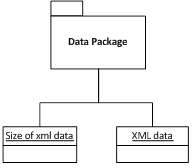
\includegraphics[scale=0.8]{XMLDataPackageFigure}

\caption{Image of the data sent between the EIS environment and the agent controller.\label{fig:DataPackaging}}


\end{figure}


This was done to ensure that the agent controller at all times knew
how much data was to be transmitted, thus giving it the right to deny
packages if they were over a certain size. In our current implementation
however no package size is denied. 


\subsubsection*{Engine Side of EIS Support}

In the project: \texttt{XmasEngineExtensions }we provide two classes:
\begin{description}
\item [{\texttt{EISAgentController:}}] this class is responsible for converting
xml data from the EIS environment into actions that can be queued
to the agent it controls. And also for converting percepts the agent
it controls receives into XML data that can be sent to the EIS environment.
\item [{\texttt{EISAgentServer}}] creates a TCP server all EIS environments
that wishes to connect to it must make a TCP client call, once a connection
is established then the agent server will construct an \texttt{EISAgentController
}object, that object will take over all further duties of comuncation.
\end{description}

\subsubsection*{How the EISAgentServer works}

The server manages the agent controllers and it also manages the connection
creation between an EIS environment and an \texttt{EisAgentController}.

On Fig. \ref{fig:EISServerSequenceDiagram} is shown how an EIS environment
connects to an agent server and how the agent server handles the connection.
The connection works by the EIS environment making a TCP connection
request the agent server then responds by constructing the agent controller(
and give it, its own thread). Once the agent controller is constructed
the agent server is no longer responsible for handling that connection
and leaves it up to the agent controller to find out what the EIS
environment wants. This is basically to connect to a given agent whom
it knows by name, and start sending it actions.

\begin{figure}
\begin{centering}
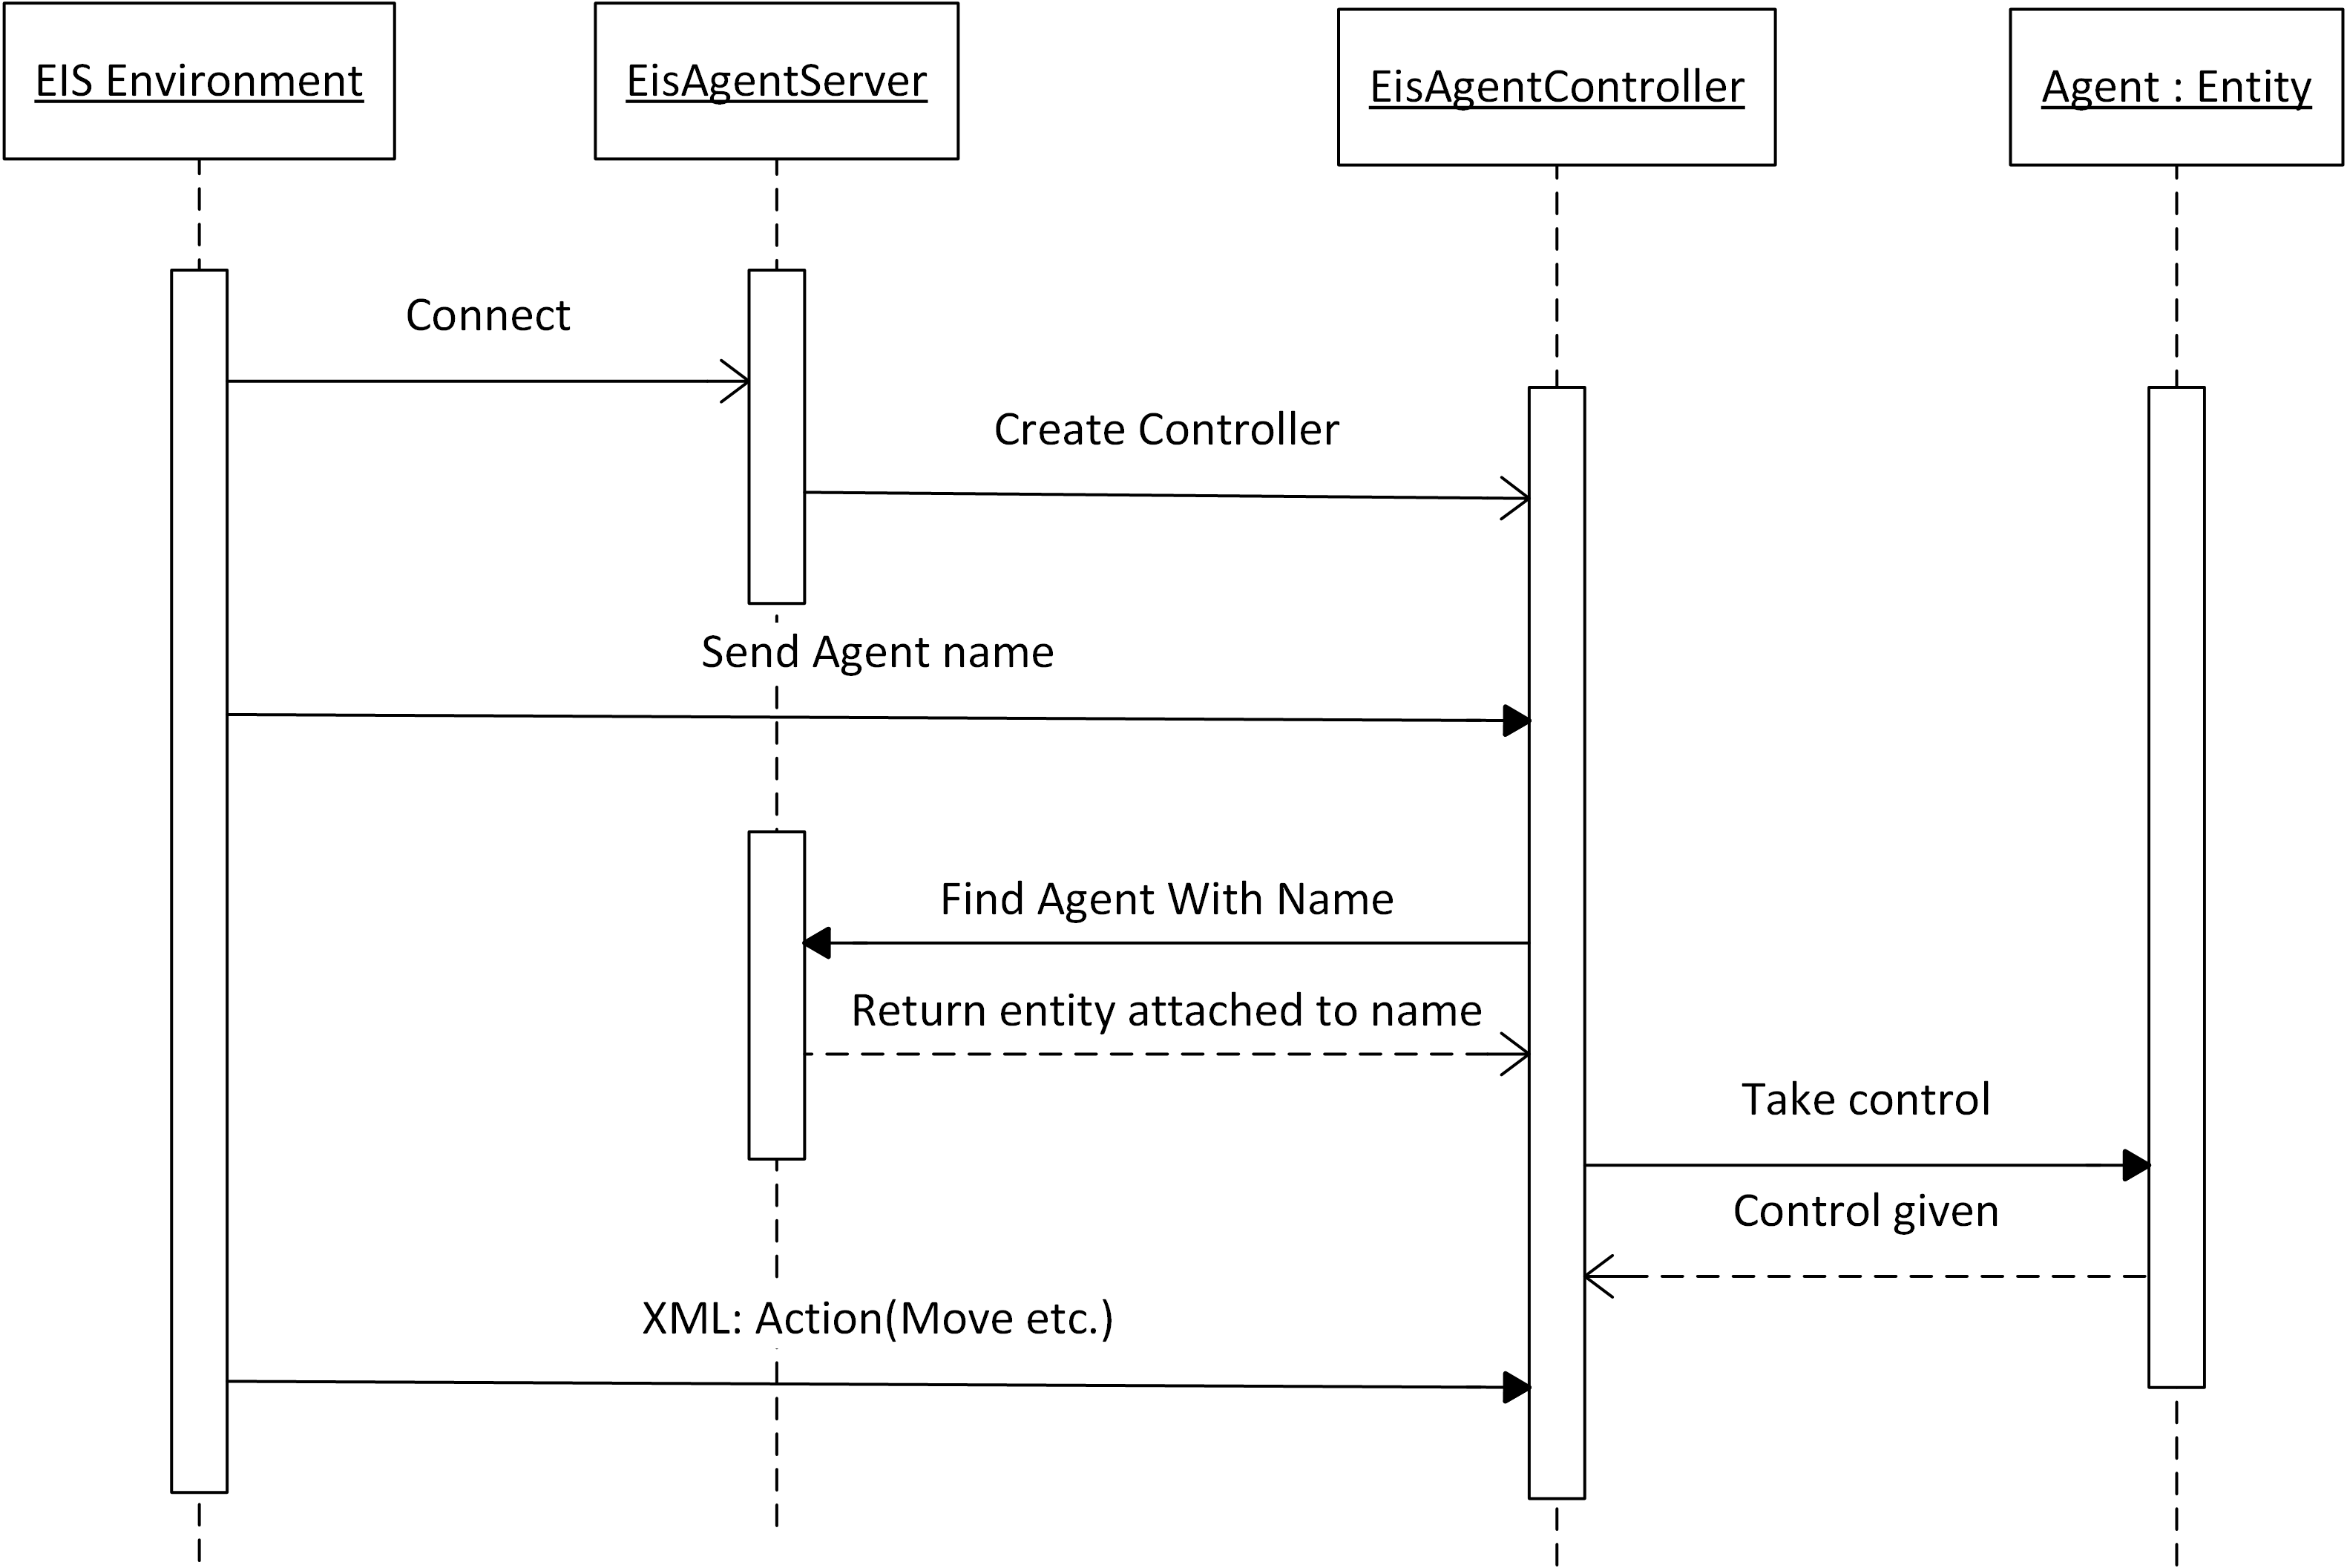
\includegraphics[width=1\textwidth]{EISServerSequenceDiagram}
\par\end{centering}

\caption{a sequence diagram of an EIS environment connecting to the engine
through an EisAgentServer.\label{fig:EISServerSequenceDiagram}}


\end{figure}



\subsubsection*{How the EisAgentController works}

The EIS agent controller job is to ensure that all demands made by
an EIS environment is fulfilled, this is done by receiving actions
in XML data form, and convert the data into Xmas Actions. These actions
are then queued onto an agent.

\begin{figure}
\begin{centering}
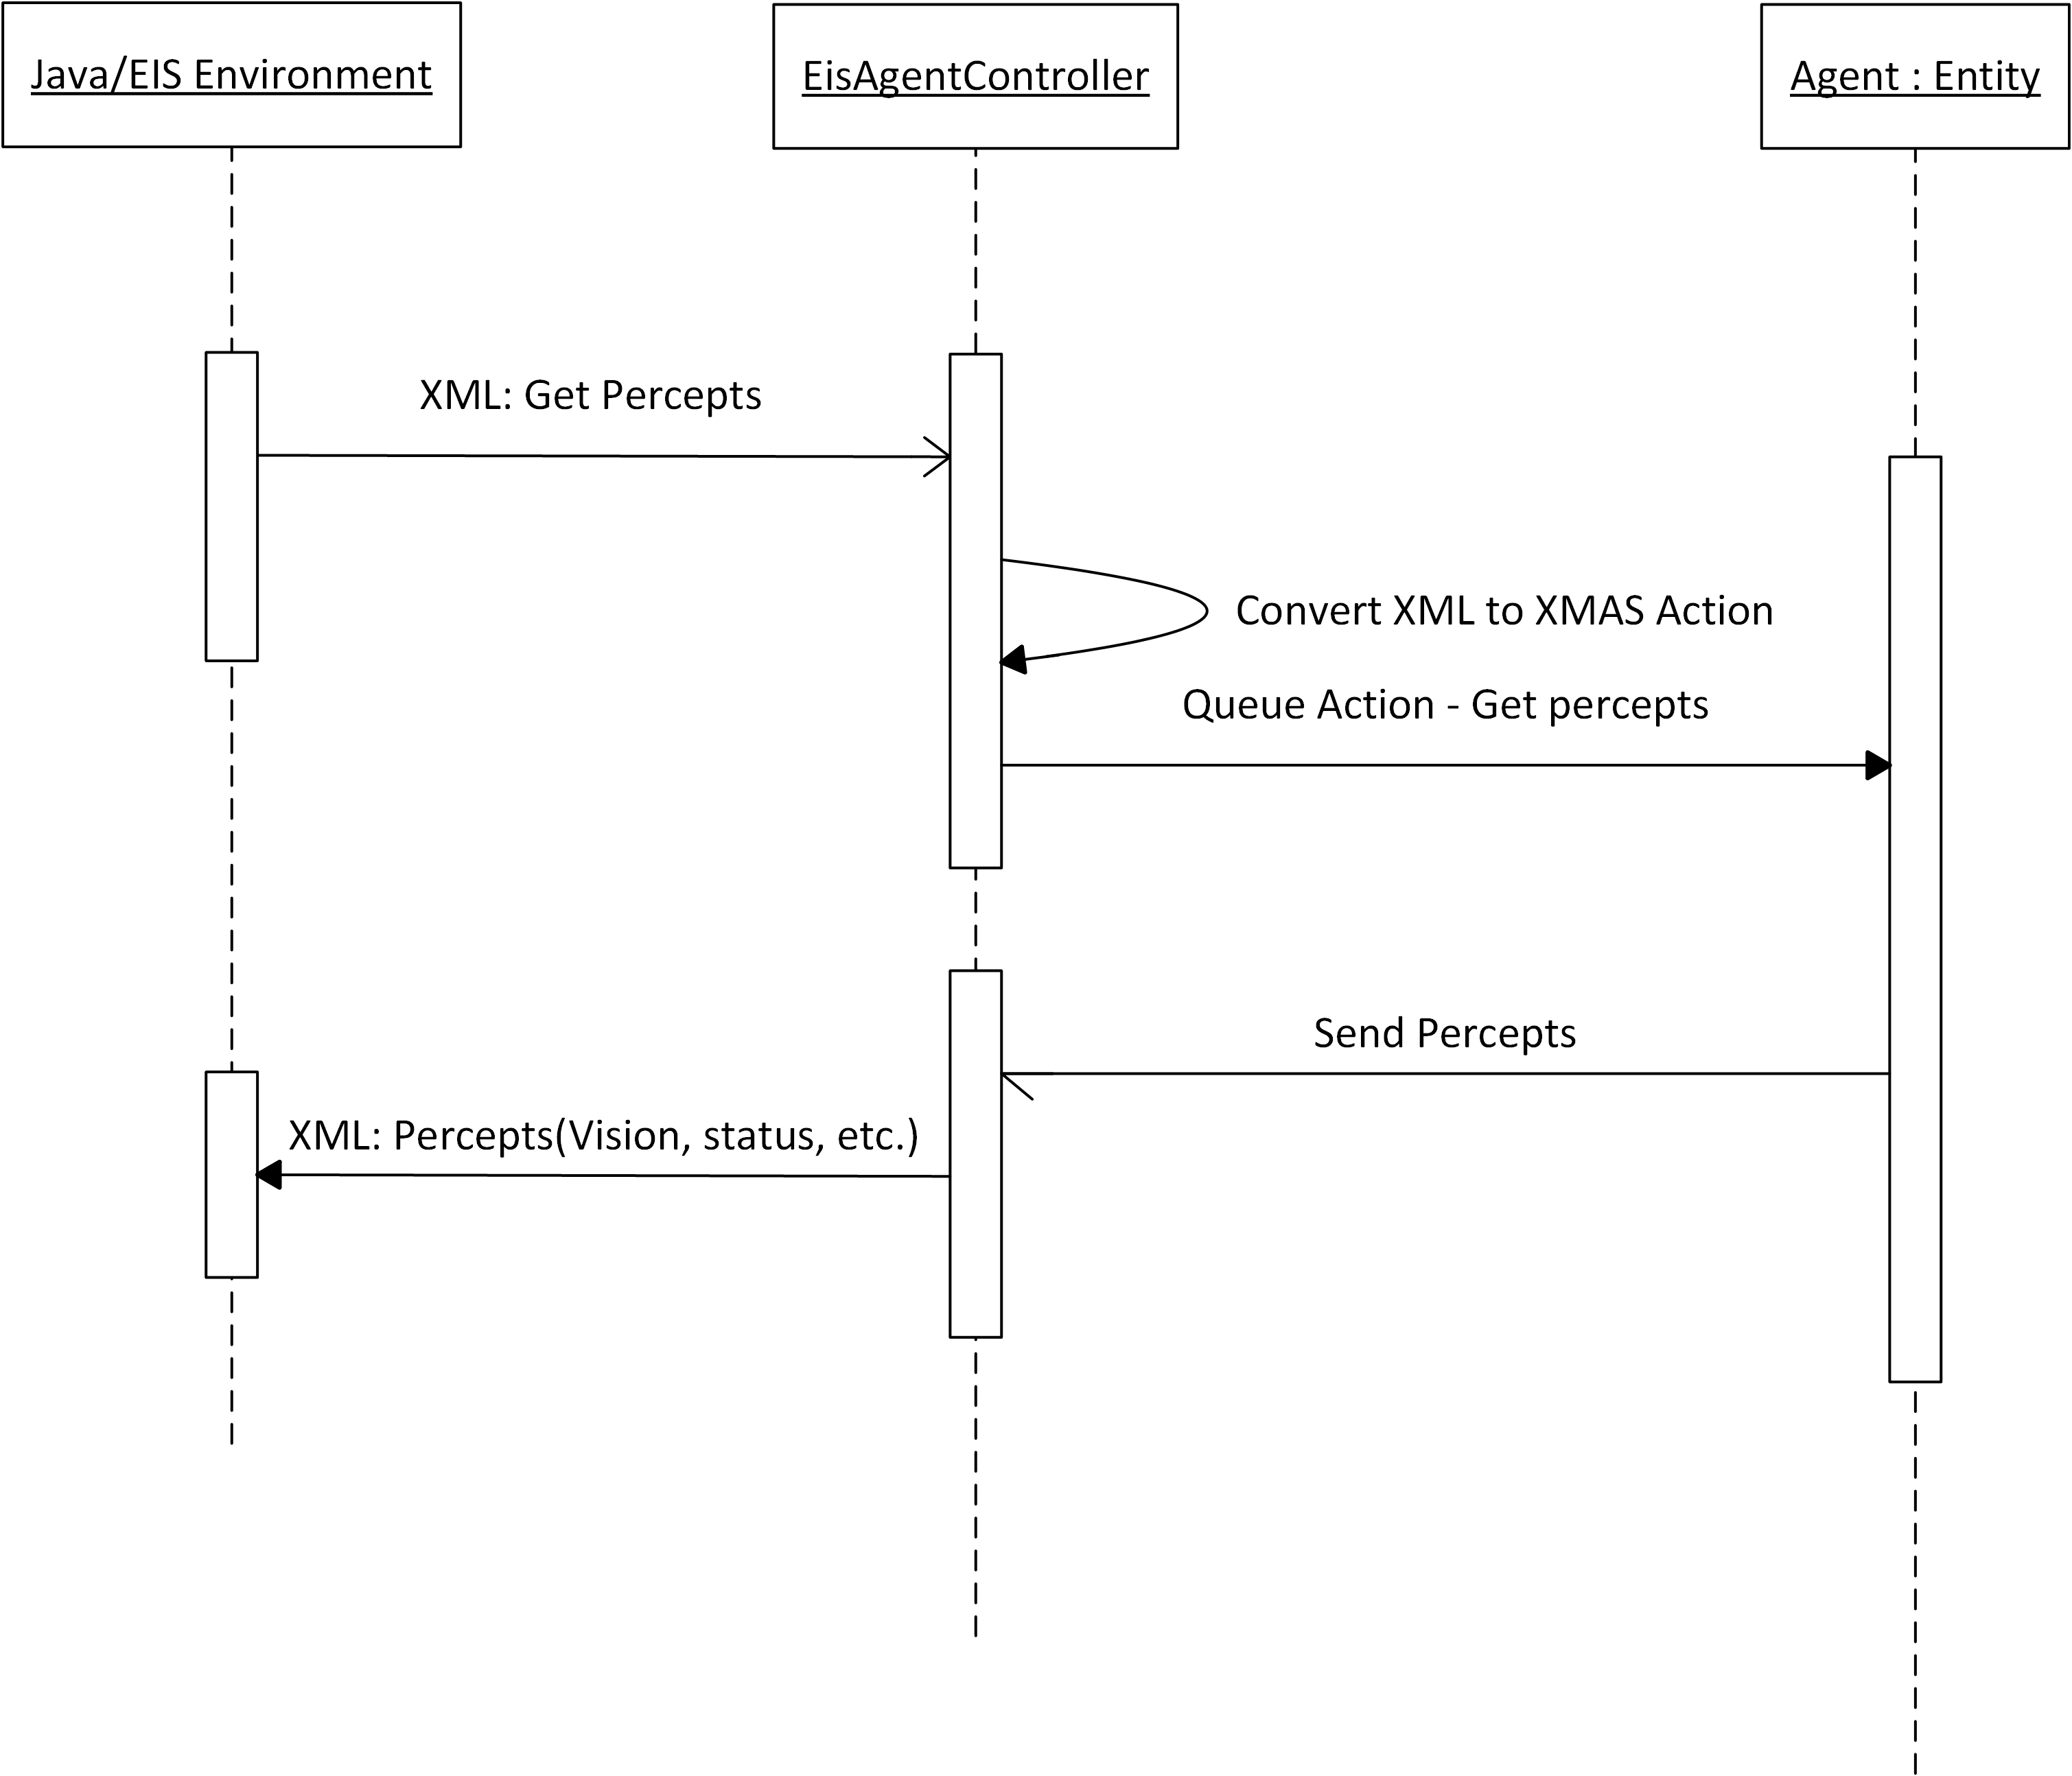
\includegraphics[width=1\textwidth]{EisAgentControllerSequenceDiagram}
\par\end{centering}

\caption{A sequence diagram showing how XML data from EIS environment are converted
into Xmas data.\label{fig:EisAgentControllerSequenceDiagram}}


\end{figure}


On fig. \ref{fig:EisAgentControllerSequenceDiagram}, is shown how
xml data received is converted by the controller and then sent to
the agent inside the engine. Percepts are only sent if they are updated
in this case the action was to get percepts however if the action
was to move an agent, then no percepts would be sent the controller.


\subsubsection*{EIS Environment}

The EIS environment is designed to setup an interface between an APL
and an environment built in java. As our engine is built In C\#, we
cannot use the EIS as it was supposed to. The way we use EIS instead
is by making it a hollow link between our engine and the APL(such
as GOAL). Thus the EIS environment implementation we make must be
able to provide communication between the APL and our engine. The
way we have done this is by making the environment convert all the
XML data it receives into the EIS data-structures for percepts. Which
is one of the classes that EIS provides, it all provides the means
to directly convert the data structures into prolog code which is
used by GOAL to understand the data.

\begin{figure}
\begin{centering}
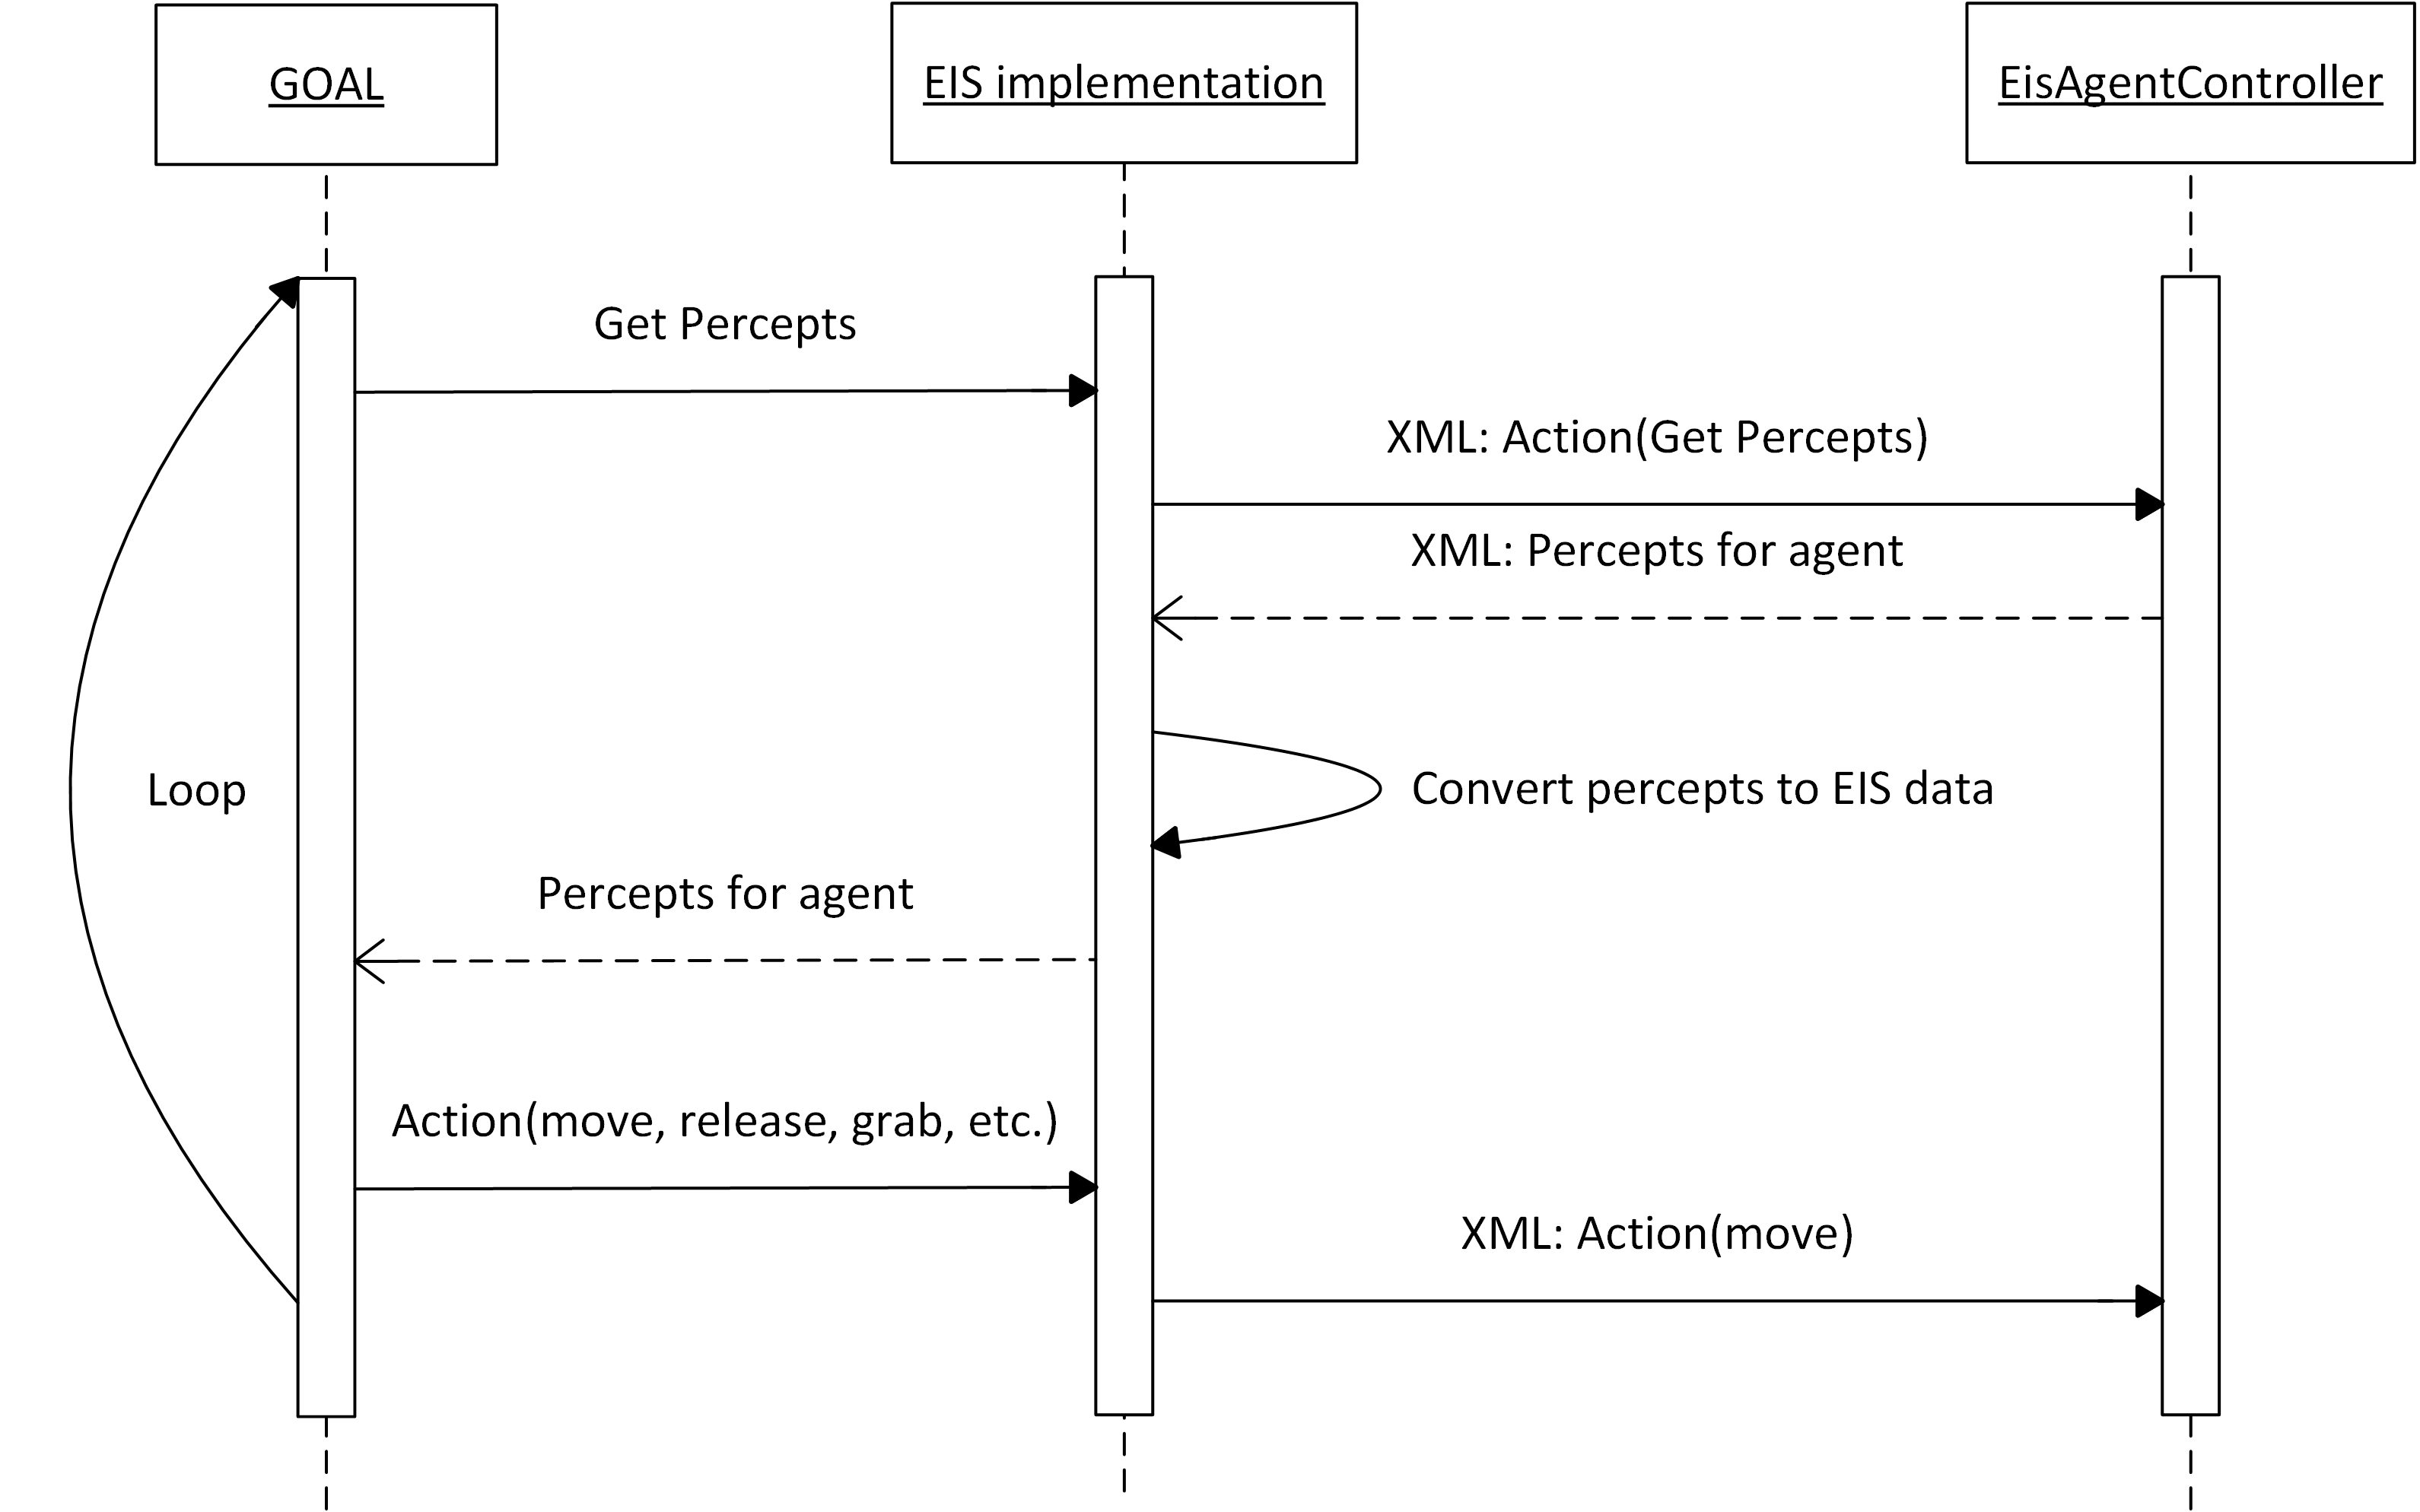
\includegraphics[width=1\textwidth]{EISEnvironmentToGoalSequenceDiagram}
\par\end{centering}

\caption{This diagram shows how the communication between goal and the EIS
environment works.\label{fig:EISEnvironmentToGoalSequenceDiagram}}


\end{figure}


An example of sequence for the EIS environment communicating with
an APL(such as GOAL) can be seen on fig. \ref{fig:EISEnvironmentToGoalSequenceDiagram}.
The basic idea is that the goal program sends commands directly to
the EIS environment we have implemented and then we ensure that those
commands are fulfilled by transmitting them over to the \texttt{EisAgentController},
through a TCP connection.


\subsection*{Considerations}

The design of interfacing with goal was originally what the engine
design was mostly focused on; as such there have been lots of different
approaches to this interfacing that we have gone through. One approach
was to connect the EIS environment using J\# which could be converted
into C\# byte code; this would be a lot faster than our current approach
since XML data wastes a lot of space by encapsulating every bit of
information. However J\# is an old language and we wanted to ensure
that we did not run into too many complications under development
as such we chose our current approach since the real time transmission
of data is not as important as the idea of it, for this project in
particular. 


\subsection*{Summary}

EIS is an interface for designing environments in java that connects
to EIS supported APLs, we use this environment to develop an environment
that is simply a TCP connection between the APL(in our case goal)
and our engine. The design provides the necessary features to the
engine, but the design could have been more optimized by using a more
compact way of sending data, since sending data as XML nodes takes
up a lot of space since XML requires all data to be encapsulated by
it.



\section{Reference Implementation}

The reference implementation relies heavily upon the extensions that
are attached as part of the engine. Thus to see how the reference
implementation was designed we would refer to look at those extensions.

The extensions the reference implementation uses:
\begin{description}
\item [{Logger~Extension}] this is used to log all actions that occur
inside the engine and to log any errors that might also occur.
\item [{EIS~Extension}] this extension is used to connect the reference
implementation to our goal program for the agents inside the reference
implementation.
\item [{Tile~World~Extension}] the reference implementation uses a Tile
based world as such it directly uses the Tile World Extension that
provides just this functionality.
\end{description}
The reference implementation as such only provides:
\begin{itemize}
\item Actions specific to the reference implementation(Grabbing/releasing
packages)
\item Entities specific to the reference implementation(Walls, Player, etc.)
\item Percepts and modules specific to the reference implementation(Holding
package percept)
\item A view in console form
\item A Goal program
\item A way to control an agent with keyboard
\end{itemize}

\subsection{The Console View}

The console view is designed is optimized to draw the screen at a
specific frame rate. When the console view does not draw it will instead
update all view data is has stored.

To change view data in a view, an event must be fired from the model,
however since the model is operating on a different thread than the
view. The view must ensure no concurrent errors. This is done by using
the \texttt{ThreadSafeEventMananger}, as explained in \ref{ImplementationView}.

\begin{figure}
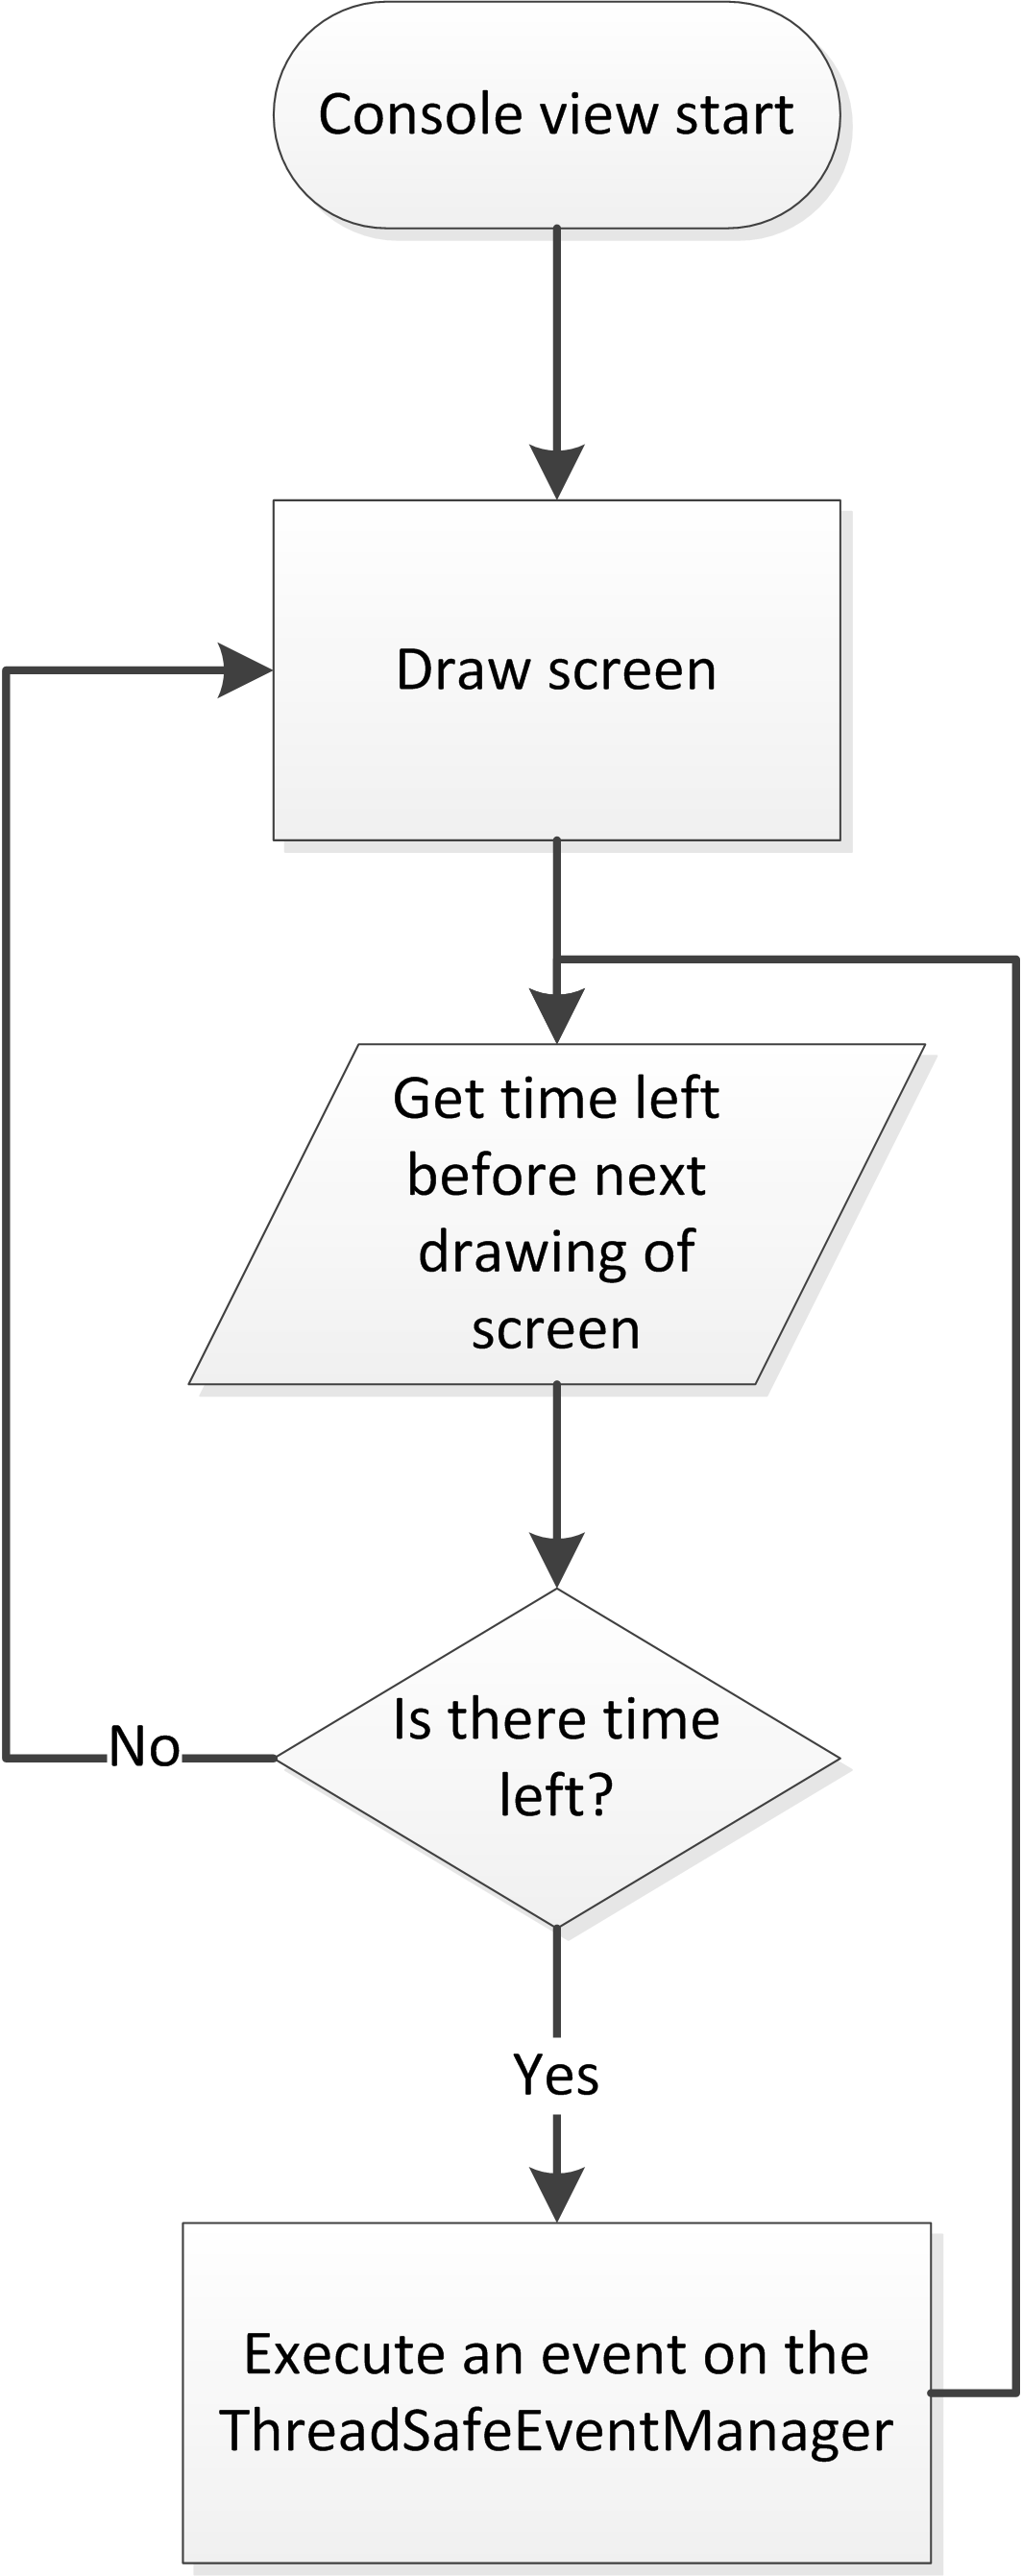
\includegraphics[width=0.4\textwidth]{ConsoleViewDrawingFlowChart}

\caption{the sequence of the console view drawing process\label{fig:FlowOfConsole}}


\end{figure}


The console view works by drawing the screen, then if it has time
between left before the next drawing is scheduled the view will execute
a single event on the \texttt{ThreadSafeEventManager}. The view will
continue this process until either, there is no events left to be
executed or the time is up and it is time for it to perform the next
drawing of the screen. On fig. \ref{fig:FlowOfConsole} a drawing
of this process can be seen.

This provides the reference implementation with a very quickly updated
view as no time is wasted on the thread and instead will continue
to update even when it is not drawing. Furthermore by updating the
view data in a separate thread the engine core does not use its computation
power on handling this making the engine overall more efficient.


\subsection{GOAL Program Implementation}

The goal program is designed to work directly with our reference implementation,
as it is just a show case of how such a program might look like, it
will make assumptions based on how the reference implementation interact.
For instance it will assume that there are entities called walls that
are meant to block off tiles. 

To see the source code of our goal program commented, look in appendix
\ref{GoalCodeAppendix}.


\subsubsection{Agent Decision}

A full flow chart of the goal program decision chart can be found
on appendix \ref{GOALFlowChartAppendix}.

As can be seen from the flow chart, the agent will try and find packages
and bring them to a dropzone, if no such packages can be found or
if no dropzone is found, the agent will start exploring the entire
world.

The goal program operates with a few different notions; 
\begin{description}
\item [{Street}] the first notion is the notion of streets. A tile is a
street if it contains no wall types such a normal walls or impassableWalls(map
boundary walls) this means that the agent can move on this tile.
\item [{Route}] all the agents decisions are preplanned this means that
the agent determines where to move to, this plan is put into a route,
the agent will follow this route whenever it has nothing else to do,
such as grabbing/releasing packages.
\end{description}
\begin{figure}
\begin{centering}
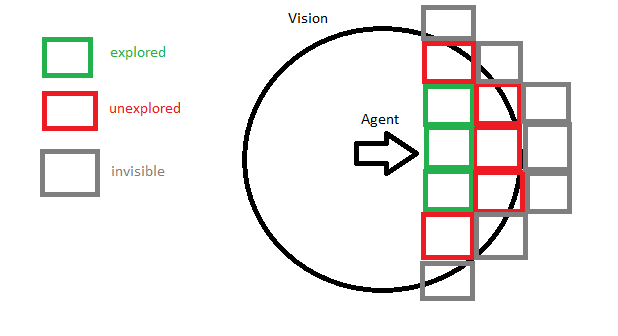
\includegraphics[width=0.8\textwidth]{VisionExploredGOALAgent}
\par\end{centering}

\caption{An image of an agent\textquoteright{}s vision and which it would determine
to be explored\label{fig:VisionExploredGoalAgent}}
\end{figure}

\begin{description}
\item [{Explored}] the agent\textquoteright{}s goal is to eventually have
all tiles explored as this means that all packages has been collected
from the world. The agent determines that a tile has been explored
if it has seen all its adjacent tiles. This works great for the agent
because until it reaches a wall the unexplored tiles that it has stored
as a street will always be considered unexplored, no matter how far
it moves, this makes the agent work much like putting a carrot in
front of a mule, no matter how much the agent explores whenever it
explores something, there is always something new that becomes unexplored.
As such this will continue until a wall has been reached on all its
paths. \\
A tile is determined to be explored if all tiles adjacent to has been
seen by the agent, fig. \ref{fig:VisionExploredGoalAgent} shows an
image of this.
\end{description}

\subsection*{Summary}

The reference implementation was designed as a reference for all the
features of the engine, as such it made heavily use of the extensions
that we implemented. This section only covered the view and the goal
program in details. This is because most of the reference implementation
consists of either declaring new agent/entity types or wiring all
the extensions together, as such there was almost no business logic
involved which makes them rather uninteresting to explain in detail.

One part that the reference implementation does not cover which could
have been interesting was the notion of linked module as explained
in \ref{SysFeatEntities}. This could have been used in the reference
implementation but we did not choose to do so.

Overall the design of the reference implementation is very solid and
fulfills the goals we had for it, which were to be a showcase for
our engine.



\chapter{Testing}

\texttt{\emph{{[}Missing{]}}}


\subsection{Unit Testing}

\texttt{\emph{{[}Missing{]}}}



\chapter{Discussion}

In this section we will discuss the major considerations we faced
during the project, as well as the choices we took in accomplishing
our goals, and how we could have otherwise reached them.


\section{Generality of the engine}

One of the major goals of this project was to make the engine as general
as possible. This includes the ability for the designer to implement
any kind of environment, displayed any way he wants, and controlled
by whatever APL he would like to use. In this section we will discuss
how these three vital parts of our engine lives up to this goal.

For the engine to be general means it has the ability to adapt to
any needed situation. The only restriction is that these situations
are based on Multi agent Environment, other than that nearly any situation
should be coverable by the engine. For instance if one wishes to use
the engine to make a computer game, then the view must be able to
support a graphical display and the world of the engine must have
the ability to be changed to a 3d-world. But if instead one wishes
to make an engine for searching documents for spelling errors, then
the world should be extendable to a text-document. Furthermore to
be general also means that the engine should be used to work with
any other APL, so regardless if the APL is goal, Jason or F\# the
engine should have the ability to be adapted into working with either
of those languages.

In many cases, the shortest path to a general system is removing restrictions.
Unfortunately, features are often restrictive in nature; the most
general system of all is one that is completely featureless. Thus,
it is often a trade-off between features and generality.


\subsection*{Model}

For the model to be general, it should be capable of representing
a world as any possible data structure. Additionally, the objects
inhabiting it should be as general as possible, allowing them to be
defined in a way that makes sense in the context of the world. 

We have accomplished this by imposing as few restrictions as possible
on these objects. For example, as described in section \texttt{\emph{{[}System
Features.World{]}}}, a world in the engine has no data associated
with it by default, leaving the modelling of it completely in the
hands of the designer. The only restriction on the world is the idea
that all entities should have a postition in it, although the position
object is completely general itself. \texttt{\emph{{[}Environments
where postition does not matter?{]}}}

Initially, we toyed with the idea of equipping the world with a graph
as the default representation of the environment, since it is a very
general data structure in the sense that it can be used to describe
other data structures. The problem with this approach is that a graph
may not be the best representation of any given world. In the case
of a tile based world, for example, a two dimensional array is more
feasible, since this is its natural representation. Ultimately, we
chose to impose no restrictions on the data structure used, and instead
rely on the use of extensions to model environments.


\subsection*{Interfacing with APLs}

One of the major problems in designing an interface that works with
different APLs is that the order in which they queue actions and queries
percepts may be different from APL to APL. In effect, they do not
share a common execution protocol. This means that we cannot provide
a general method for communicating with any AP. Instead, as with other
parts of the engine, the intent is to allow for extensions capaple
of interfacing with different APLs in any way they see fit.

It could be argued that using the notions of percepts and actions
serves to limit the universality of the engine. These are, however,
general concepts for interacting with an intelligent agent. They are
basically the input and output of the agent; it perceives the state
of the world, and produces an action based on this information. \texttt{\emph{{[}Explain
why the functions of an agent can not be reduced any further (why
they are the basis for an agent), refer to AIMA{]}}} As such, they
are essential to interacting with an agent, and incorporated in all
agent programming languages we are aware of.


\subsection*{View}

For the view to be considered general it is paramount that the design
of the view is not being restricted in anyway, this is done by keeping
anything in the view very minimalistic. By minimalistic we mean that
the view only provides about four classes and they only provide a
little about of business logic. If we had narrowed down how exactly
a view should be designed such as requiring a frame for which the
view is projected on. This might have made implementations of the
view easier as tools to draw on frames could be pre-implemented into
the engine. We did not want to do this since we think that restrictions
should be non-existent .However this also poses a potential problem
in that it is so minimalistic that we barely provide anything for
the user, and leave the user to the task of making the view by themself.


\subsection*{Solving the Problems of Generality}

As evident when discussing how to make the engine general and how
to make it work with as many situations as possible, the problem arises
that the workload for the user gets increased. This is because whenever
we remove something from the engine in order to ensure that we impose
no restrictions, we run the risk of removing something that made the
life of the user easier, since they would not have to re-implement
it themself. To combat this problem we moved everything that added
value to the engine but imposed a restriction to the Engine Extensions
project. The idea would be that while the extensions was not part
of the core engine, they would be part of what we delivered with the
engine. We saw this as the best of both worlds, not only do we ensure
that the engine is not being restricted, but at the same time if the
user did not mind some restrictions, then they would be able to find
a suitable extension among the ones we provide. As of now the only
extensions we have are those needed for the reference implementation,
but our long term plan would be to add more extensions if possible.


\section{Model View Controller Design Pattern}

The model view controller design pattern is one of the older design
patterns within software design; its purpose is to ensure that the
developer does not deal with multiple issues at once, and instead
is able to focus on one task of the project at a time. We chose to
base our engine on the MVC pattern because we also do not want the
user of the engine to be tasked with multiple issues at once. Without
the MVC pattern, the user could be confused about how for instance
they should design a controller for an APL, and perhaps they would
mistakenly design it tailored to specific actions. If the user did
this, they would have to write new actions to perform the same task
for each new APL they encountered, which would increase code redundancy.
As the designers of this engine we wanted to ensure those kinds of
mistakes do not happen. The way we enforce this is by forcing the
MVC pattern. Since by forcing the MVC pattern we force the user to
think about how they should construct the implementation of the engine\textquoteright{}s
abstract classes. However since it is only a pattern, the user can
still make bad design decisions as we impose no restrictions. As most
bad design decisions comes from making an easy implementation of something,
we hopefully reduce the number of times they are made by making bad
decisions harder. \texttt{\emph{{[}rewrite sentence?{]}}}


\section{Choice of Technologies}


\subsection*{The XMAS Engine}

We have chosen to implement the engine in C\#, which runs on the .NET
platform. While Java has a strong presence in multi-agent system development
-- as it is used by established APLs such as Jason, as well as the
EIS standard -- we have a subjective preference for C\#. In general,
C\# is a newer and more modern programming language with better facilities
for writing comprehensive and maintainable code, and provides some
features usually only found in functional programming languages. Additionally,
.NET code can be executed across platforms, thanks to the Mono project%
\footnote{\texttt{http://www.mono-project.com}%
}, although the newest version of .NET (v4.5) has not been ported at
the time of this writing. Although developing our reference implementation
would have been simpler had we used Java, opting out of this in favor
of C\# gave us the opportunity to test how well our engine interfaced
with programs not written in the same language. 


\subsection*{Reference Implementation}

As our reference implementation was developed to showcase and test
our engine, we aimed to implement it using the most commonly used
agent programming language. Since EIS can be interfaced with many
different APLs, this seemed like the obvious choice. If the engine
could be shown to work with EIS, any APL supported by EIS would work
by extension. Initially, we considered writing a J\# (.NET bindings
for the Java Language) module, which would work natively with both
our engine written in C\#, and the EIS implementation written in Java.
However, we felt that this would remove the difficulties of communicating
with an entirely different platform. This difficulty is important
to face, since 


\section{Comparison to other Environment Construction Tools}

In this section, we will compare the XMAS engine to other frameworks
that can be used to construct and manage MAS environments. In particular,
we will consider CArtAgO%
\footnote{\texttt{http://cartago.sourceforge.net/}%
} (\emph{C}ommon ``\emph{Art}ifacts for \emph{Ag}ents'' \emph{O}pen
framework, henceforth referred to as Cartago), which have been used
in several projects, and as a part of the \emph{JaCaMo}%
\footnote{\texttt{http://jacamo.sourceforge.net/}%
} (\emph{Ja}son, \emph{Ca}rtago, \emph{Mo}ise) project, which provides
a complete framework for multi-agent systems consisting of the Jason
MAPL (multi-agent programming language), the Cartago environment constructions
API, and the Moise organizational system. We will also compare our
engine to using plain EIS.


\subsection{Cartago}


\subsubsection*{Agents and Artifacts}

The Cartago framework uses the \texttt{A\&A} (Agents and Artifacts)
approach to designing environments. In the following, we will provide
an overview of this model, which is presented in ~\cite{Ricci08}.

In the A\&A meta-model, a collection of computational entities called
\emph{artifacts} constitutes the environment. They are computational
entities in the sense that they are meant to provide functionality
exploitable by the agents, and can have a state and business logic,
but are not meant to act autonomously. In fact, instead of agents
having predefined actions that manipulates the state of the world
when executed, they are aware of a collection of artifacts, which
each provide a number of operations the agents can perform on them.
The artifacts also provides percepts to the agents, and are as such
the agents' means of interacting with the world. 

Artifacts can not only be used to model objects with a physical presence
in the world (such as analogues to the packages and dropzones in our
reference implementation), but also more abstract concepts, such as
control flow objects. For example, a communication artifact could
be created, through which several agents could talk and listen, through
operations and percepts, respectively. Since agents can create and
destroy artifacts at will, such communication channels are easy to
spawn in an ad hoc manner.

The A\&A meta-model, as described in ~\cite{Ricci08}, is to some
extent based on the way humans interact in a working environments,
as it draws on research in fields such as organisational sciences
and anthropology. This lead to the introduction of artifacts as tools,
service providers and communication devices, since they better describe
such an environment. In general, the A\&A approach focuses on incorporating
these concepts as an integral part of the environment, so as to make
it a functional and reactive part of a multi-agent system. This is
in contrast to classical MAS engineering, where the environment is
typically defined as a more static structure can act in and retreive
percepts from.


\subsubsection*{Cartago Implementation}

The Cartago framework is implemented in Java and can natively connect
to the Jason APL. Here, we will explain how Cartago implements the
A\&A meta-model. A more thorough explanation can be found in ~\cite{Ricci11}.
\begin{description}
\item [{Agents}] In Cartago, agent programs are connected to agent bodies,
which are -- in that respect -- conceptually similar to agent controllers
in the XMAS engine, as they represent a vessel for the agent in the
environment, but no agent logic. In keeping with the A\&A approach
explained above, the agent API allows for creating and deleting artifacts,
as well as executing operations on artifacts and retreiving percepts
from them. 
\item [{Sensing}] For handling perception, Cartago provides the concept
of \emph{sensors}. An agent contains a set of sensors, each collecting
percepts from an artifact. The \texttt{sense} method of an agent takes
a sensor as input and returns a percept gathered by it, whereafter
the percept is removed from the sensor. The sensors can be overridden
by the designer to -- for example -- control in what order it should
return its contained percepts. A sensor is connected to an artifact
via the \texttt{focus} method. Sensory inputs can be filtered, so
that a sensor only picks up percepts matching a user-defined pattern.
\item [{Artifacts}] Artifacts specify operations that agents can execute
as described by the A\&A meta-model. Artifacts can generate events,
which can be gathered by any connected agent sensors. Artifacts can
describe how they are meant to be used, ie.\ what operations thay
have and how they should be called. When an agent executes an operation
on an artifact, a boolean value is immediately returned, signifying
either success or failure. The calling agent can give a sensor as
an argument to the method invocation, which will gather any percepts
that the artifact generates as a result of executing the operation.
\end{description}

\subsubsection*{Agents and Artifacts in XMAS}

The main purpose of the Cartago project is to provide a framework
for designing MASs using the A\&A meta-model. While that have not
been the goal of the XMAS engine, it is general enough to support
this approach, especially since the engine allows entities to incorporate
state and business logic through entity modules. Below, we have described
how artifacts, agents and perception would be implemented using the
engine:
\begin{description}
\item [{Agents}] would be XMAS agents, with a module for creating, destroying
and containing (references to) artifacts, as well as a module for
each sensor. The \texttt{sense} action used in the Cartago API is
not entirely equivalent to our generic \texttt{getAllPercepts} action,
as it only retrieves one percept from one specific sensor, but such
an action could easily be implemented. 
\item [{Artifacts}] would be represented as entities with a module for
each operation the artifact provides. When new stimuli, ie.\ new
percepts, would be available, an XMAS event would be raised.
\item [{Sensing}] The agents' sensor modules would be connected to the
artifact entities by registering triggers on them, wchich would subscribe
to the events raised by the artifacts. By using trigger conditions
(cf. section \texttt{\emph{{[}Events and triggers section{]}}}), the
percepts could be filtered as with Cartago sensors. The modules in
XMAS already provides means for being queried for collections of percepts,
so this functionality could be used to let them return all the percepts
that have become available to them since the last invocation. Alternatively,
they could incorporate some logic for the ordering of returned percepts,
in case the user only wants one percept per \texttt{sense}.
\end{description}
The functionality described above could be encapsulated in an engine
extension, providing the proper modules, events and actions. One issue
with this is that entities in the XMAS engine are meant to have a
position. As mentioned, this is not a strict requirement, as the position
can be set to a null value and ignored. Additionally, recent versions
of Cartago supports what they call workspaces, which serves to group
the agents and artifacts together in different sub-environments, for
which positions in the XMAS engine would be well suited.


\subsection{Environment Interface Standard}


\subsubsection*{}



\chapter{Conclusion}

\texttt{\emph{In this project, we have developed an engine for constructing scenarios
to be used in multi-agent systems. A scenario in this sense is an
environment where agents can interact, and with means to control the
agents. Our project provides the following features:
\begin{itemize}
\item A way to set up environments.
\item Means of communicating with APLs, which controls the agents inhabiting
the environment.
\item Provide a general way for agents to behave in the environment, by
allowing them to \emph{act} and \emph{sense}.
\item Reactivity in the environments, allowing agents and entities to dynamically
respond to changes in the world.
\end{itemize}

\section{Results of comparisons}

As discussed in \ref{sec:DiscussionComparison}, our engine is placed
somewhere in between Cartgo and EIS in terms of multi-applicability
and features. That is, our engine is more general than Cartago, while
providing more convenient features for a MAS than EIS (and is, conversely,
less feature complete than Cartago). We have argued that the meta-model
used in the Cartago project can be implemented in Xmas, and shown
that EIS can be used as an extension to the engine in order to exploit
its APL compatibility.


\section{Engine completion}

We will now evaluate whether the goals we listed in the introduction
have been reached:
\begin{description}
\item [{Generality:}] As we discussed in section \ref{sec:DiscussionGenerality},
we believe we have reached a good amount of generality in the engine,
as we impose few restrictions on the design of environments. The eternal
problem is the trade-off between generality and features, and much
of our effort have been directed towards equalizing these two qualities.
Without several implementations of the engine, it is difficult to
say how well our solution caters to different environment systems
and their needs.
\item [{Ease~of~use:}] While our engine features tools that can ease
the development of larger systems, it is not comparatively easier
to use in small scale apllications. Our minimal example implementation
(Vacuum World, see Appendix \ref{chap:VacuumWorldAppendix}) consists
of a total of 17 C\# classes. It should be noted, however, that the
example does not use any extensions apart from the very basic logger
extension. Extensions can be used to define some of the abstract notions
such as position, and thus ease the development burden. It is also
worth noting that most of the classes contains very little code.
\item [{Cross~platform~compatibility:}] We have compiled the project
against the mono platform, which provides the .NET platform on Mac,
Linux and Windows. We have developed the engine in both Linux and
Windows, and it works as it should on both platforms. At the moment,
our reference implementation can not be run on Linux or Mac due to
a bug in Mono regarding text buffer sizes when printing to a terminal.
While the reference implementation is an important part of this project,
we do not consider it a part of the core of the Xmas engine, and therefore
conclude that this goal has been reached.
\end{description}
In summation, we believe that the goals for the engine have mostly
been reached.

However, There are many aspects of the engine which could be severely
improved. These include, but is not limited to, 

\textbullet{} The specific way actions and events are designed. For
instance, the distinction between environment events and entity events,
as discussed in section \ref{sub:ImplementationEventsTriggers}.

\textbullet{} The way the view is supposed to communicate with the
model

\textbullet{} The way agent controllers are forced to have their own
threads. This is unnecessary when APLs runs all agents on a single
thread, however inefficient that may be.


\section{Future work}

Here, we will list some of the possible additions to the engine, which
would make it easier to use by providing functionality for a wide
array of MAS scenarios.
\begin{itemize}
\item Extensions to communicate with other APLs, that do not support the
EIS standard.
\item A collection of common environments, such as:

\begin{itemize}
\item Three dimensional worlds
\item A graph based world
\end{itemize}
\item An extension allowing construction and management of discrete worlds.
\item Extending the reference implementation to include agents cooperating
to find packages. 
\item Copying the environment and functionality of the Agents on Mars scenario,
to showcase and test our engine against an established implementation.
\item A collection of commonly used agent actions and percepts, such as
means of communicating with each other.\end{itemize}

}}
\appendix
\chapter{Stuff}

This appendix is full of stuff ...                                 %Appendix A
%-----------
% Backmatter
%-----------
\backmatter
\chaptermark{Bibliography}
\renewcommand{\sectionmark}[1]{\markright{#1}}
\sectionmark{Bibliography}
\addcontentsline{toc}{chapter}{Bibliography}        %Force addition of Bibliography to TOC
\bibliographystyle{alpha}                           %Use alpha codes for references
\bibliography{References}                           %Bibliography file called
\end{document}
% % % EOF % % %